%\PassOptionsToPackage {warpHTML,BaseJobname=SprManual}{lwarp}
%\documentclass[pdflatex,a4paper,ja=standard,jafont=ipaex]{book}
\documentclass{book}

\usepackage{iftex}

% --- LOAD FONT SELECTION AND ENCODING BEFORE LOADING LWARP ---

\ifPDFTeX
  %\usepackage[whole,autotilde]{bxcjkjatype}
  \usepackage[whole]{bxcjkjatype}
  \usepackage{lmodern}            % pdflatex
  \usepackage[T1]{fontenc}
  \usepackage[utf8]{inputenc}
\else
  \usepackage{fontspec}           % XeLaTeX or LuaLaTeX
\fi

% --- LWARP IS LOADED NEXT ---
\usepackage[
%   HomeHTMLFilename=index,     % Filename of the homepage.
%   HTMLFilename={node-},       % Filename prefix of other pages.
%   IndexLanguage=english,      % Language for xindy index, glossary.
%   latexmk,                    % Use latexmk to compile.
%   OSWindows,                  % Force Windows. (Usually automatic.)
%   mathjax,                    % Use MathJax to display math.
]{lwarp}
% \boolfalse{FileSectionNames}  % If false, numbers the files.

% --- OTHER PACKAGES ARE LOADED AFTER LWARP ---
\usepackage{makeidx} \makeindex
%\usepackage{xcolor}             % (Demonstration purposes only.)

\usepackage{graphicx, booktabs, amsmath, amssymb, url, makeidx, color}
\usepackage{lwarp_macros, fancybox, framed, longtable, bm, comment}
\usepackage{ifthen, setspace}

\usepackage{dirtree}
%\usepackage{setspace}
%\usepackage{longtable}

\ifLwarp\else
  \usepackage{atbegshi}
  \AtBeginShipoutFirst{\special{pdf:tounicode EUC-UCS2}}
  %\AtBeginShipoutFirst{\special{pdf:tounicode 90ms-RKSJ-UCS2}}
  \usepackage{bookmark}
\fi
\usepackage{hyperref,cleveref}  % LOAD THESE LAST!

% --- LATEX AND HTML CUSTOMIZATION ---
%\title{The Lwarp Tutorial}
%\author{Some Author}
%\setcounter{tocdepth}{1}        % Include subsections in the \TOC.
%\setcounter{secnumdepth}{1}     % Number down to subsections.
\setcounter{FileDepth}{1}       % Split \HTML\ files at sections
%\booltrue{CombineHigherDepths}  % Combine parts/chapters/sections
%\setcounter{SideTOCDepth}{1}    % Include subsections in the side\TOC
%\HTMLTitle{Webpage Title}       % Overrides \title for the web page.
%\HTMLAuthor{Some Author}        % Sets the HTML meta author tag.
%\HTMLLanguage{en-US}            % Sets the HTML meta language.
%\HTMLDescription{A description.}% Sets the HTML meta description.
%\HTMLFirstPageTop{Name and \fbox{HOMEPAGE LOGO}}
%\HTMLPageTop{\fbox{LOGO}}
%\HTMLPageBottom{Contact Information and Copyright}
\CSSFilename{lwarp_sagebrush.css}



\title{Springhead - How to use CMake}
\date{}

\renewcommand{\figurename}{Fig.\,}
\renewcommand{\tablename}{Table\,}

\begin{document}
\maketitle
\tableofcontents
\listoffigures

% macro.tex
%	Last update: 2019/10/03 F.Kanehori

\makeatletter

%% alias for fonts
\let\it@\it
\let\tt@\tt
\let\bf@\bf
\let\rm@\rm
\let\gt@\gt
\let\mc@\mc
\def\it#1{{\it@{#1\,}}}
\def\tt#1{{\tt@{#1}}}
\def\bf#1{{\bf@{#1}}}
\def\rm#1{{\rm@{#1}}}
\def\gt#1{{\gt@{#1}}}
\def\mc#1{{\mc@{#1}}}
\def\Use@font#1#2{%
	\if#1t\tt{#2}\else
	\if#1i\it{#2}\else
	\if#1b\bf{#2}\else
	\if#1r\rm{#2}\else
	\if#1g\gt{#2}\else
	\if#1m\mc{#2}\else\rm{#2}\fi\fi\fi\fi\fi\fi}

%% make local scope
%
\def\LocalScope{\begingroup}
\def\endLocalScope{\endgroup}

%% dimensions
\newdimen\WID \WID=20pt		% standard indent width

%% spaces
%  \Vskip{amount}
%  \Hskip{amount}
%	amount		amount of skip (dimen)
%
\def\Vskip#1{\begin{Vmode}\vspace{#1}\end{Vmode}}
\let\Hskip\hspace

%% force vertical mode
%  \begin{Vmode} ... \end{Vmode}
%
\def\Vmode{\ifvmode\relax\else\par\hrule width 0pt height .5\baselineskip\fi}
\def\endVmode{\relax\par}

%% ruler / underline
%  \thinrule{width}
%
\def\thinrule#1{\rule{#1}{0.1pt}}

%% quoted word
%

\ifLwarp
\def\SQuote#1{`#1'}
\def\DQuote#1{"#1"}
\def\KQuoteS{``}
\def\KQuoteE{''}
\def\KQuote#1{``#1''}
\else
\def\SQuote#1{\hspace{0pt}\Quote@{`}{#1}{'}}
\def\DQuote#1{\hspace{0pt}\Quote@{"}{#1}{"}}
\def\KQuoteS{\hbox{\hbox{\ \raise.4ex\hbox{``}}}}
\def\KQuoteE{\hbox{\hbox{\raise.4ex\hbox{''}}}}
\def\KQuote#1{\hspace{0pt}\Quote@knj{\,#1}}
\fi
\def\Quote@#1#2#3{\hbox{\,\raise.4ex\hbox{{\tt #1}}#2\raise.4ex\hbox{{\tt #3}}\,}}
\def\Quote@knj#1{\hbox{\,\raise.4ex\hbox{``}#1\,\raise.4ex\hbox{''}}}

%% abbreviations
%
\def\Dagger{$\dagger$}
\def\DDagger{$\ddagger$}
\def\CDots{$\cdots$}
\def\LDots{$\ldots$}
\def\VDots{$\vdots$}
\def\Yen{Y\llap=}		% yen sign

%\def\Note#1{\hbox to 1.5em{\raise1ex\vbox{\scriptsize{#1}}}}
\def\Note#1{\raisebox{1ex}{{\scriptsize #1}}}

%% some specific ones
%
\def\Cont{\ \ {\rm{\scriptsize{(���̍s�ɑ���)}}}}
\def\Path#1{\DQuote{\tt{#1}}}
\def\PathBgn#1{\hbox{\,\raise.4ex\hbox{{\tt "}}\tt{#1}}}
\def\PathEnd#1{\hbox{\tt{#1}\raise.4ex\hbox{{\tt "}}\,}}

%% make framed box to denote some command
%  \CmndBox{body}
%  \Cmnd{body}
%	indent		amount of indentation from left margin
%
\def\CmndBox#1{%
	\begin{LocalScope}\vskip .3\baselineskip
	\noindent\hbox{%
		\framebox[\linewidth][t]{%
			\def\arraystretch{.8}\tabcolsep=5pt%
			\tt{\begin{tabular}{l}#1\end{tabular}}}}%
	\vskip .3\baselineskip
	\end{LocalScope}}

\def\Cmnd#1{%
	\vbox{\vskip .4\baselineskip\CmndBox{#1}\vskip 0\baselineskip}}

%% narrower
% \narrow[size][margin]
%	charsize:	t, f, s, [n]
%	margin:		[\the\leftmargin]
% \end{narrow}
%
\def\narrow{\@ifnextchar[{\narrow@}{\narrow@def[Z][\the\leftmargin]}}
\def\narrow@[#1]{%
	\@ifnextchar[{\narrow@def[#1]}{\narrow@@[#1]}}
\def\narrow@@[#1]{%
	\ifx#1t \def\@size{t}\def\@mgn{\the\leftmargin}\else
	\ifx#1f \def\@size{f}\def\@mgn{\the\leftmargin}\else
	\ifx#1s \def\@size{s}\def\@mgn{\the\leftmargin}\else
	\ifx#1n \def\@size{n}\def\@mgn{\the\leftmargin}\else
	\ifx#1l \def\@size{l}\def\@mgn{\the\leftmargin}\else
		\def\@size{Z}\def\@mgn{#1}\fi\fi\fi\fi\fi
	\narrow@def[\@size][\@mgn]}
\def\narrow@repl#1{\def\@lmgn{\the\leftmargin} \def\@text{[#1]}}
\def\narrow@same#1{\def\@lmgn{#1} \def\@text{}}
\def\narrow@def[#1][#2]{%
	\if#1t \def\font@def{Y}\let\font@size\tiny	   \else
	\if#1f \def\font@def{Y}\let\font@size\footnotesize \else
	\if#1s \def\font@def{Y}\let\font@size\small	   \else
	\if#1n \def\font@def{Y}\let\font@size\normalsize   \else
	\if#1l \def\font@def{Y}\let\font@size\large	   \else
	\if#1Z \def\font@def{Y}\let\font@size\relax	   \else
	       \def\font@def{N}\let\font@size\relax	   \fi\fi\fi\fi\fi\fi
	\if\font@def Y \narrow@same{#2} \else \narrow@repl{#2} \fi
	\begin{Vmode}%
	%\vspace{.25\baselineskip}%
	\list{}{\topsep 0pt \partopsep 0pt \parsep 0pt \itemsep 0pt
		\rightmargin 0pt \leftmargin \@lmgn \relax}\item[]
	\begingroup\font@size\@text}
\def\end@narrow{\endgroup\endlist\end{Vmode}}
\let\endnarrow\end@narrow


%% CMake specific abbreviations
%
\def\Anno#1{\rm{\footnotesize{ \CDots\  #1}}}
\def\SolutionFile{�\�����[�V�����t�@�C��\raise1ex\hbox{{\tiny [*1]}}}
\def\ProjectFile{�v���W�F�N�g�t�@�C��\raise1ex\hbox{{\tiny [*2]}}}
\def\cmake{\tt{cmake}}
\def\make{\tt{make}}
\def\SprLib{Springhead���C�u����}
\def\SprProj{Springhead�v���W�F�N�g}
\def\VS{Visual Studio}

\def\SprTop#1{\Path{C:/Springhead{#1}}}
\def\AppTop#1{\Path{C:/Develop/Application{#1}}}
\def\build{{\it{build\/}}}

\def\CMakeLists#1{\Path{CMakeLists.txt{#1}}}
\def\CMakeOpts#1{\Path{CMakeOpts.txt{#1}}}
\def\CMakeConf#1{\Path{CMakeConf.txt{#1}}}
\def\CMakeTopdir#1{\Path{CMakeTopdir.txt{#1}}}

\makeatother

% end: marco.tex


\chapter{Springhead Library�̓���}
\label{InstallingSpringheadLibrary}
% 1.0.Install.tex
%	Last update: 2020/02/13 F.Kanehori
\newpage
\section{インストール}
\label{sec:Install}
\parindent=0pt

この章では、\SprLib のダウンロード及びビルドの方法について説明します。

\medskip
\SprLib は、Windowsおよびunixの両方のプラットフォームに対応しており、
ビルド環境はCMakeを用いて生成します
(WindowsではVisual Studio用のsolution file / project file、unixでは\tt{Makefile})。

\Important{%
	Visual Studio 2015/2017用のsolution file / project fileも配布していますが、
	今後のバージョンアップに対応することを期待しないでください。}

% end: 1.0.Install.tex

% 1.1.Download.tex
%	Last update: 2020/02/10 F.Kanehori
%\newpage
\subsection{ダウンロード}
\label{subsec:Download}
\parindent=0pt

\SprLib はGitHubで管理されており、
次のURLからダウンロードすることができます。
\bf{以下、ダウンロードするディレクトリを\SprTop{}として説明を進めます。}

\CmndLine{%
	> chdir C:/Springhead\\
	> git clone --recurse-submodules\Cont\\
	\Hskip{100pt}https://github.com/sprphys/Springhead
}{command-1-1-a.eps}{DownloadTree1}
\medskip

デフォルトでpythonが利用できる環境であればサブモジュールbuildtoolは必要ありません。
また、外部パッケージboost, glew, glut, glui を別途インストールして使用するのであれば
サブモジュールdependencyは必要ありません。
そのような場合には、次のようにしてサブモジュールを選択してください。

\CmndLine{%
	> chdir C:/Springhead\\
	> git clone https://github.com/sprphys/Springhead\\
	> git submodule update --init --checkout buildtool\\
	> git submodule update --init --checkout dependency
}{command-1-1-b.eps}{DownloadTree2}

\medskip
Windows exploreならば右クリックでGUIが利用できます。
Git clone の画面で recursiveにチェックを入れると
サブモジュールも一緒にダウンロードできます。

\begin{narrow}[15pt]
	\begin{figure}[h]
	\begin{center}
	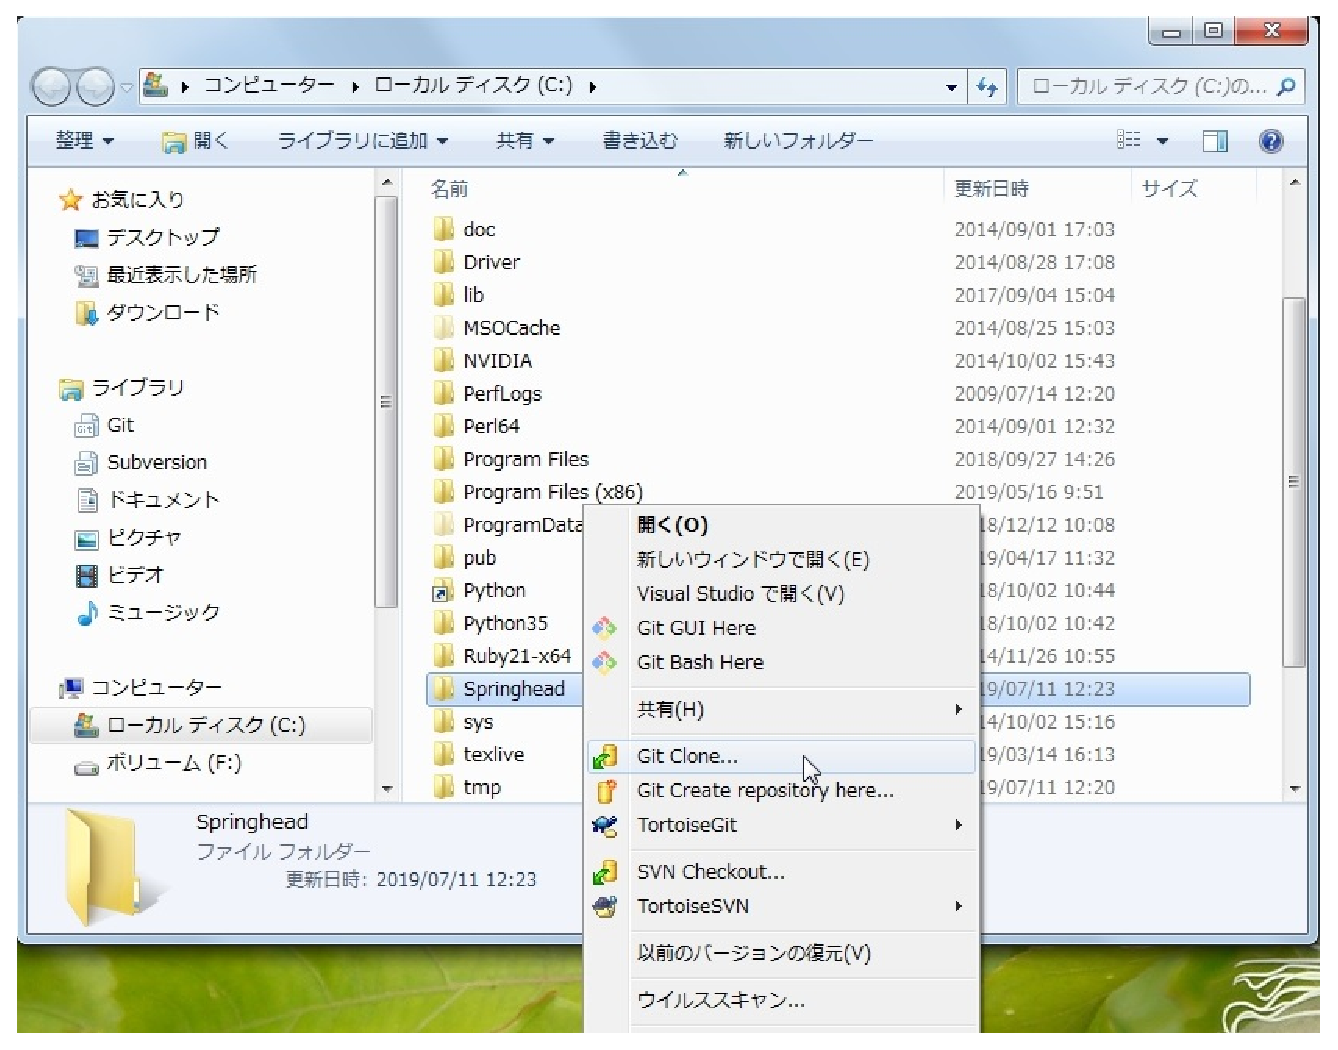
\includegraphics[width=0.5\textwidth]{fig/SpringheadClone1.eps}
	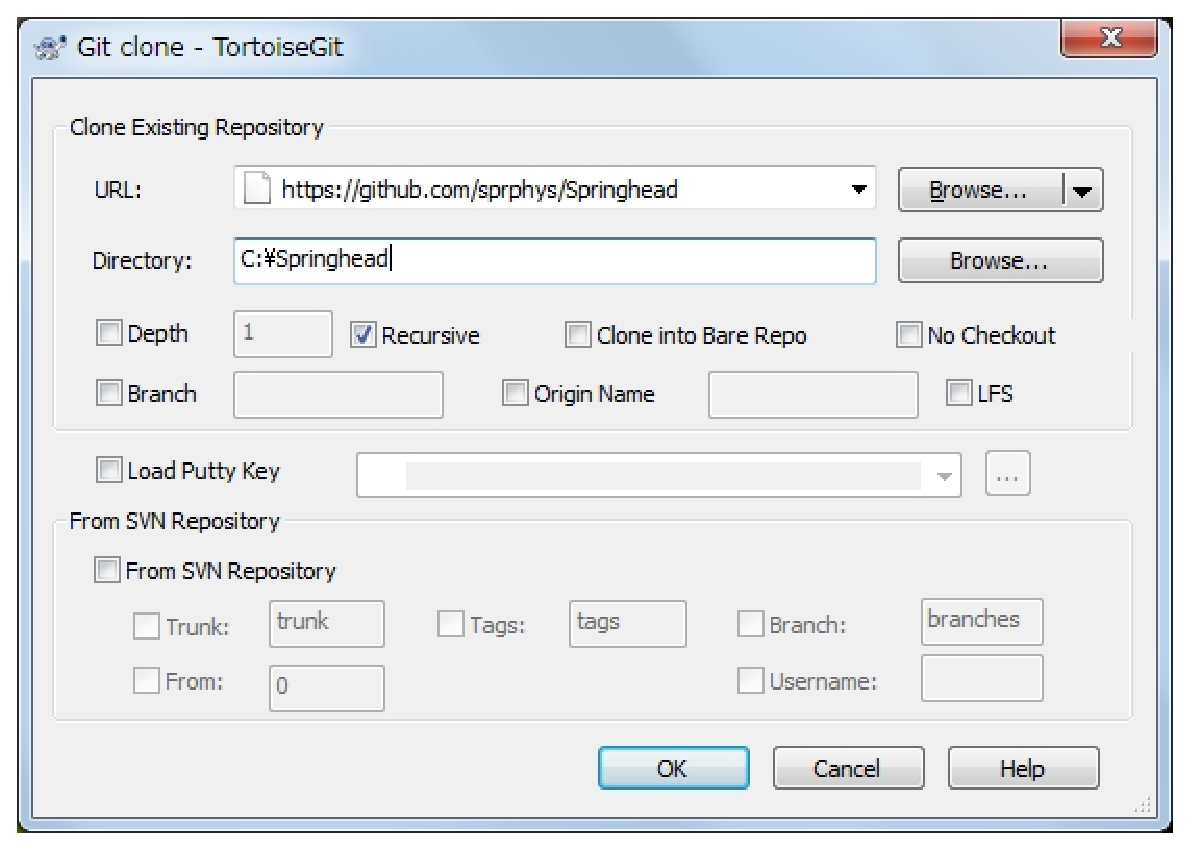
\includegraphics[width=0.4\textwidth]{fig/SpringheadClone2.eps}
	\end{center}
	\caption{Springheadダウンロード}
	\label{fig:SpringheadClone}
	\end{figure}
\end{narrow}

\Important{%
	サブモジュールを導入するのに必要なディスク容量は、
	buildtoolが約32MB、dependencyが約550MBです。}

\newpage

% end 1.1.Download.tex

% 1.2.Preparation.tex
%	Last update: 2020/02/13 F.Kanehori
%\newpage
\subsection{ビルドの準備}
\label{subsec:Preparation}
\parindent=0pt

ダウンロードが済んだら、ディレクトリ\SprTop{/core/src}に移動してください。

ライブラリのビルドに関連する配布ファイルは次のものです。

\begin{center}
\begin{tabular}{l@{\hspace{5pt}$\cdots$\hspace{5pt}}l}\hline
	\tt{CMakeLists.txt.dist} & ライブラリ生成用設定ファイル \\
	\tt{CMakeSettings.txt.dist} & ビルドパラメータ変更用ファイル \\
	\tt{CMakeOpts.txt.dist} & デフォルトビルドパラメータファイル \\
	\tt{CMakeConf.txt.dist} & 外部パッケージ・インストール先設定用ファイル \\\hline
\end{tabular}
\end{center}

\bigskip
配布されたファイル\QCMakeLists{.dist}を\QCMakeLists{}という名前でコピーします。

\CmndLine{%
	> chdir C:/Springhead/core/src\\
	> \it{copy} \CMakeLists{.dist} \CMakeLists{}
}{command-1-2-a.eps}{\CMakeLists{}}

\medskip
配布されたビルド条件で問題なければ、これで準備は終了です。
\KQuote{\ref{subsec:Build} ビルド}へ進んでください。

\bigskip
独自にインストールしたパッケージ boost, glew, freeglut, gluiを使用する場合
およびライブラリファイルとヘッダファイルのインストール先を指定する場合には、
配布されたファイル\QCMakeConf{.dist}を\QCMakeConf{}という名前でコピーして
必要な編集をします。
編集の方法は\QCMakeConf{}に記述されています。

\def\cite#1{\hspace{10pt}\footnotesize{#1}}
\def\somewhere{"C:/\it{somewhere}/\it{appropreate}"}
\CmndLine{%
	> \it{copy} \CMakeConf{.txt} \CMakeConf{}\\
	> \it{edit} \CMakeConf{}\\
	\hspace{20pt}:\\
	\cite{set(CMAKE\_PREFIX\_PATH "C:/somewhre/appropreate")} \\
	\cite{\hspace{20pt}\#\hspace{40pt}{(\rm{use absolute path)}}}\\
	\cite{\hspace{20pt}\#\hspace{40pt}%
		{(\rm{multiple paths must be separated by `newline' or `semicolon')}}}\\
	\cite{)}\\
	\hspace{20pt}:\\
	\cite{set(SPRINGHEAD\_INCLUDE\_PREFIX       "C:/somewhere/appropreate)}\\
	\cite{set(SPRINGHEAD\_LIBRARY\_DIR\_DEBUG   "C:/somewhere/appropreate)}\\
	\cite{set(SPRINGHEAD\_LIBRARY\_DIR\_RELEASE "C:/somewhere/appropreate)}
}{command-1-2-b.eps}{\CMakeConf{}}

\medskip
\begin{narrow}[s][20pt]
	変数\it{variable}に値\it{value}を設定するには
	\tt{set(\it{variable} "\it{value}"}) とします。
	途中に空白やセミコロンを含まない文字列ならば引用符は省略できます。
	また、\tt{\$\{\it{variable}\}}とすると他の変数の値を、
	\tt{\$ENV\{\it{variable}\}}とすると環境変数の値を参照できます。
	文字`\tt{\#}'以降はコメントです。
\end{narrow}

\bigskip
コンパイル及びリンクのオプションはファイル\QCMakeOpts{.dist}に設定されています。
これらのオプションを変更するときは、配布されたファイル\QCMakeOpts{.dist}を
\QCMakeOpts{}という名前でコピーして必要な編集をします。

\CmndLine{%
	> \it{copy} \CMakeOpts{.dist} \CMakeOpts{}\\
	> \it{edit} \CMakeOpts{}\\
	\hspace{20pt}:\\
}{command-1-2-c.eps}{\CMakeOpts{}}

\bigskip
以上で準備作業は終了です。

% end: 1.2.Preparation.tex

% 1.3.Cmake.tex
%	Last update: 2020/02/27 F.Kanehori
%\newpage
\subsection{cmake}
\label{subsec:CmakeLibrary}
\parindent=0pt

以下では、CMakeの生成物(ビルドの生成物ではありません)を格納する
作業場所(ディレクトリ)を\DQuote{\BldDir}として話を進めます
(作業場所の名前は任意で構いません)。

\medskip
CMakeにはConfigureとGenerateの2段階があります。

\medskip
コマンドプロンプトの場合は、1回のコマンドで両方を実行できます。
\Vskip{-.5\baselineskip}

\CmndLine{%
	> chdir C:/Springhead\\
	> mkdir build\\
	> cmake -B build [\it{generator}]
}{command-1-3.eps}{cmake}

\medskip
\it{generatorの}詳細は、コマンドプロンプトで\tt{cmake --help}とすると確認できます。

\it{generator}を省略した場合のデフォルトは、
Windowsの場合にはインストールされているVisual Studioの最新バージョンが、
unixの場合には\tt{Unix Makefiles}が選択されるようです。
ただし、マシンアーキテクチャは自動的には判定されません。
Windowsで64ビットマシンの場合には \tt{-A x64}を指定してください。

\begin{narrow}[s]
	\Vskip{-.2\baselineskip}\thinrule{\linewidth}\\
	\it{generator}の例\\
	\begin{tabular}{@{\hspace{5pt}}l@{\hspace{10pt}}l}
	    Windows:	& \tt{-G "Visual Studio 15 2017" -A x64} \\
	    unix:	& \tt{-G "Unix Makefiles"} \\
	\end{tabular}\\
	\Vskip{-.2\baselineskip}\thinrule{\linewidth}\\
\end{narrow}

\Vskip{-.5\baselineskip}
cmake--guiを利用する場合は、
まず、次の画面でConfigureボタンを押します。
\begin{narrow}[15pt]
	\begin{figure}[h]
	\begin{center}
	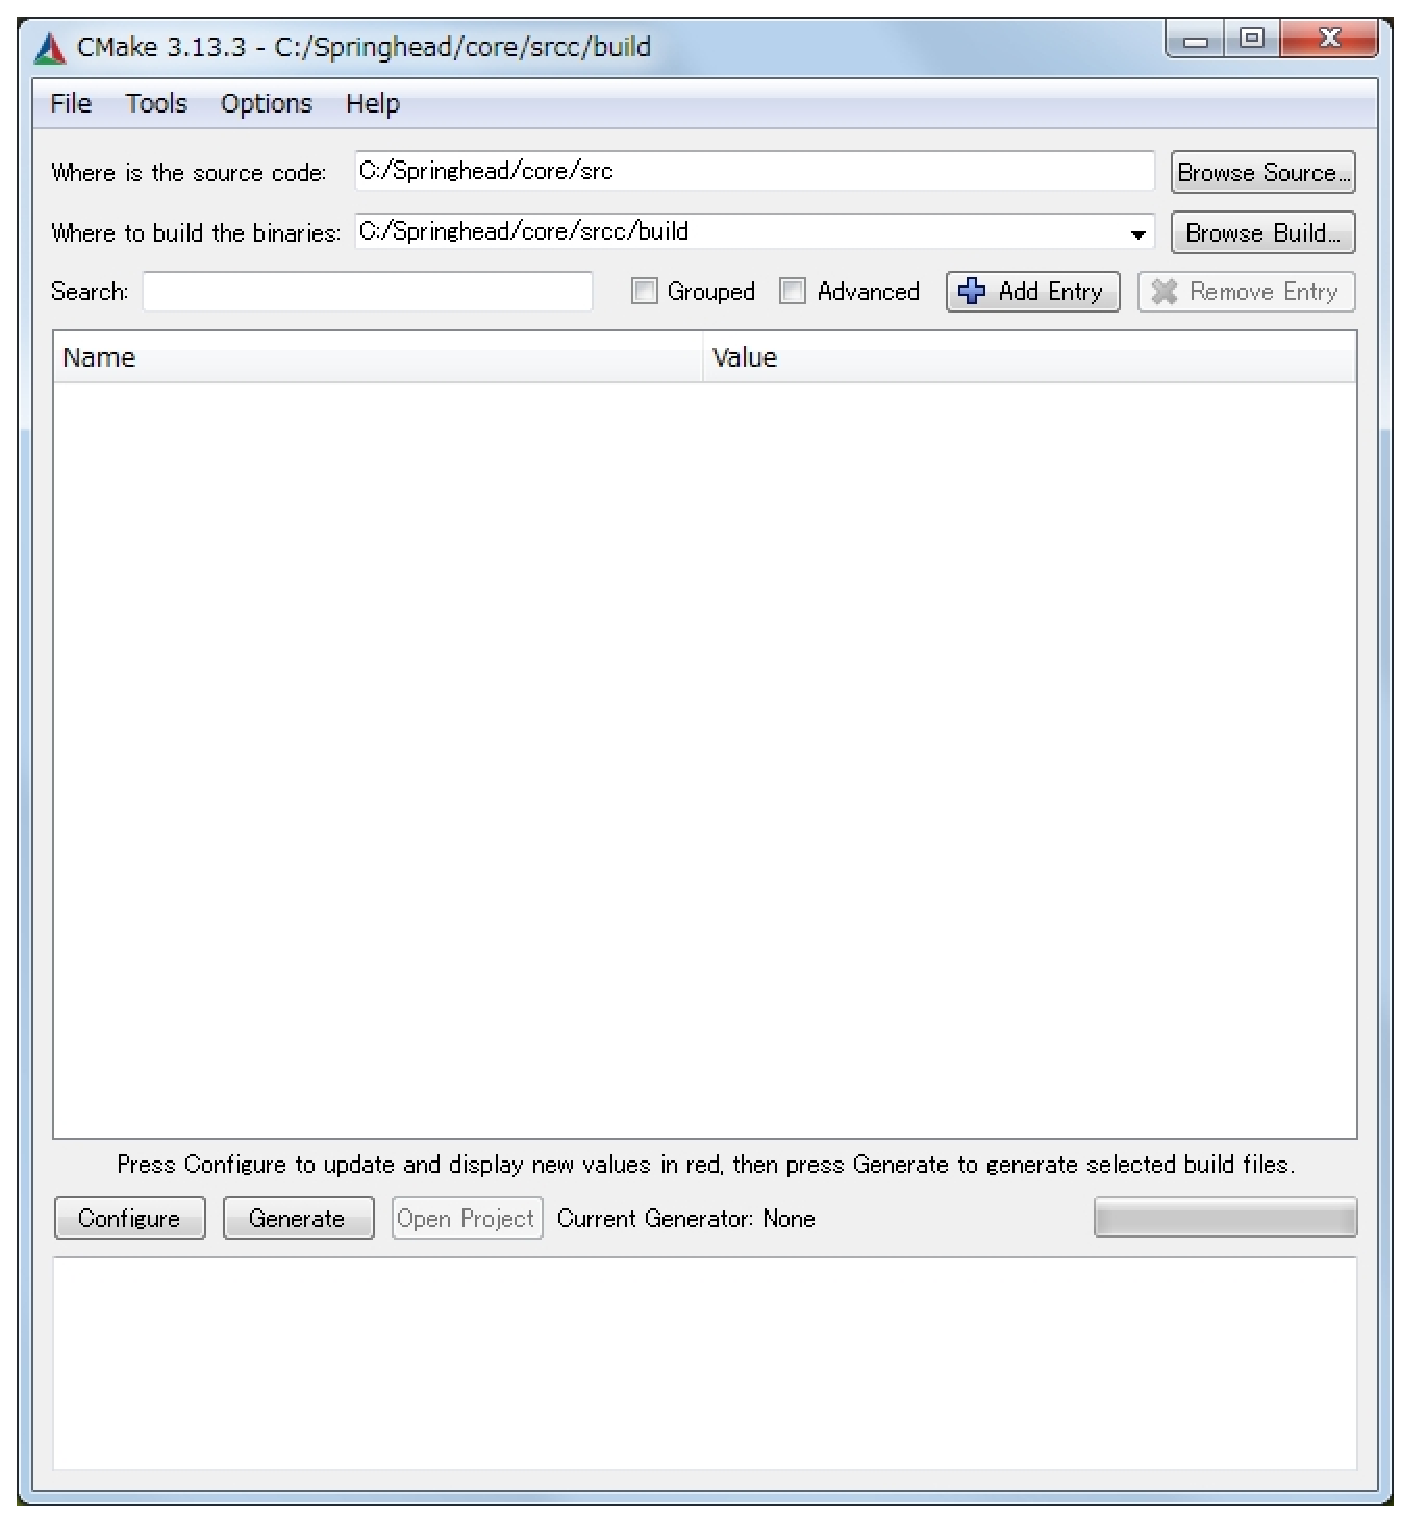
\includegraphics[width=0.7\textwidth]{fig/CmakeConfigure1.eps}
	\end{center}
	\caption{\cmake\ configure}
	\label{fig:CmakeConfigure}
	\end{figure}
\end{narrow}

\DQuote{\BldDir}ディレクトリがなければ作成するかどうかを尋ねられ、
\begin{narrow}[15pt]
	\begin{figure}[h]
	\begin{center}
	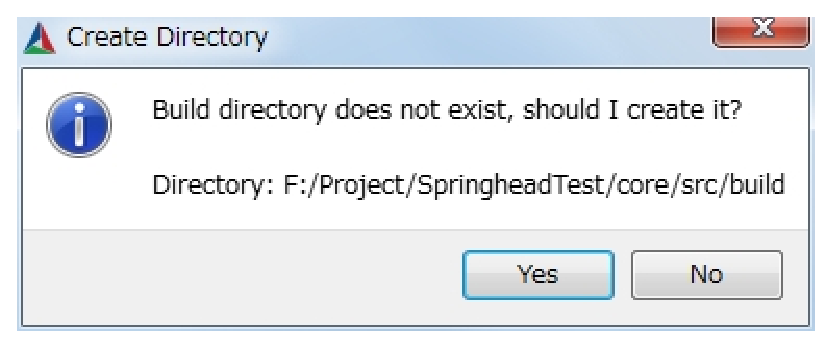
\includegraphics[width=0.5\textwidth]{fig/CmakeConfigure2.eps}
	\end{center}
	\caption{\cmake\ configure}
	\label{fig:CreateWorkSpace}
	\end{figure}
\end{narrow}

次にgenerator指定画面となります。
\begin{narrow}[15pt]
	\begin{figure}[h]
	\begin{center}
	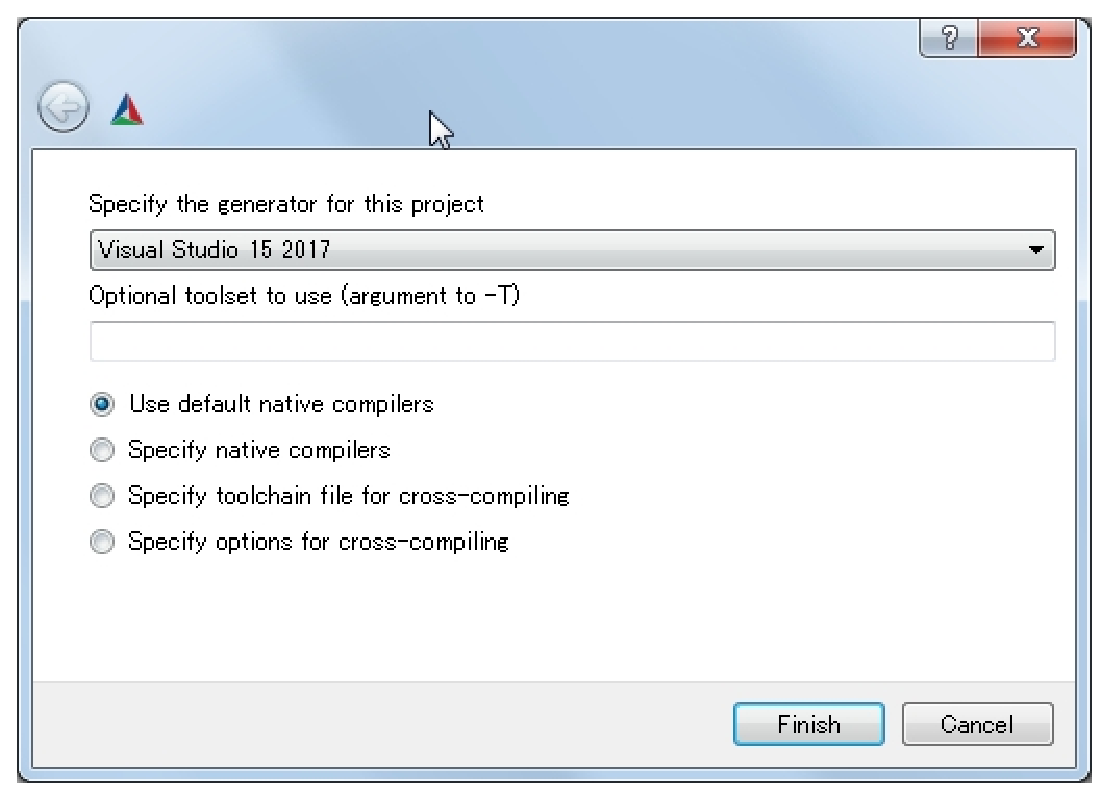
\includegraphics[width=0.6\textwidth]{fig/CmakeConfigure3.eps}
	\end{center}
	\caption{\cmake\ configure}
	\label{fig:CmakeGeneration}
	\end{figure}
\end{narrow}

最後に図\ref{fig:CmakeConfigure} のGenerateボタンを押します。

\medskip
以上で、\DQuote{\BldDir}以下にsolution file / project file (Windowsの場合)
またはMakefile (unixの場合)などが生成されたはずです。

% end: 1.3.Cmake.tex

% 1.4.Build.tex
%	Last update: 2020/02/10 F.Kanehori
%\newpage
\subsection{ビルド}
\label{subsec:Build}
\parindent=0pt

\noindent
ライブラリのビルドについては特に説明することはありません。

\medskip
\bf{Windowsの場合}
\begin{narrow}
	ディレクトリ\BldDir へ移動して\Path{Springhead.sln}をVisual Studioで実行し、
	プロジェクトSpringheadをビルドしてください。
	\KQuote{\ref{subsec:Preparation} ビルドの準備}で
	ライブラリファイルのインストール先を指定していなければ、
	ライブラリファイルは\SprTop{/generated/lib/<\it{arch}>}に生成されます。
	\tt{<\it{arch}>} はマシンのアーキテクチャに従い、
	\Path{win64}または\Path{win32}のいずれかです。
\end{narrow}

\bf{unixの場合}
\begin{narrow}
	ディレクトリ\BldDir へ移動してmakeコマンドを実行してください。
	\KQuote{\ref{subsec:Preparation} ビルドの準備}で
	ライブラリファイルのインストール先を指定していなければ、
	ライブラリファイルは\SprTop{/generated/lib}に生成されます。
\end{narrow}

% end: 1.4.Build.tex

% 1.5.EmbPython.tex
%	Last update: 2020/02/13 F.Kanehori
\newpage
\subsection{EmbPython}
\label{subsec:EmbPython}
\parindent=0pt

Python インタプリタに対する外部拡張モジュールを生成する 方法について説明します。

\Important{%
	現在作業中です。しばらくお待ちください。\\
	Windows Visual Studio用のソリューションファイルを用いてビルドする
	方法については
	\KQuote{\ref{subsec:DoNotUseCmake} CMakeを利用しない場合 (非推奨)}を
	ご覧ください。
}
\bigskip

% end: 1.5.EmbPython.tex

% 1.6.DoNotUseCmake.tex
%	Last update: 2020/02/13 F.Kanehori
%\newpage
\subsection{CMakeを利用しない場合(非推奨)}
\label{subsec:DoNotUseCmake}
\parindent=0pt

\Important{%
	この章の冒頭でも述べたとおり、
	ここで説明する方法でビルドすることは推奨しません。 
	特にWindowsの場合、
	Visual Studioの新しいバージョンに対応したファイルが配布されることは
	期待しないでください。
	また、これらのファイルはいずれ配布の対象から外される可能性がありますので、
	できればCMakeを利用するビルド環境をご利用ください。}

\bigskip
CMakeを利用しないで直接ビルドをすることもできます。
現在配布しているファイルは次のもので、\Path{C:/Springhead/core/src}に置かれています。

\medskip
\begin{narrow}[20pt]
\begin{tabular}{l@{\hspace{5pt}$\cdots$\hspace{5pt}}l}\hline
	\tt{Springhead14.0.sln} & Windows Visual Studio 2015用 \\
	\tt{Springhead15.0.sln} & Windows Visual Studio 2017用 \\
	\tt{Makefile} & unix用 \\\hline
\end{tabular}
\end{narrow}

\bigskip
\bf{Windowsの場合}
\begin{narrow}
	Visual Studio を起動し、
	"スタートアッププロジェクト"にSpringheadを指定してビルドしてください。
	ライブラリファイルは、\\
	\hspace{20pt}\Path{C:/Springhead/generated/lib/\it{arch}} \\
	に生成されます
	(\it{arch}は\Path{win64}または\Path{win32}のいずれかです)。
\end{narrow}

\bf{unixの場合}
\begin{narrow}
	\tt{make install}を実行してください。
	ライブラリファイルは、\\
	\hspace{20pt}\Path{C:/Springhead/generated/lib} \\
	に生成されます。
\end{narrow}

\medskip
\thinrule{\linewidth}

%---------------------------------------------------------------
EmbPython 関係の配布ファイルは次のものです(unix用の\tt{Makefile}はありません)。

\medskip
\bf{Springhead アプリケーションに Python インタプリタを組み込む場合}

\begin{narrow}
	Solution fileが\Path{C:/Springhead/core/src/EmbPython}に置かれています。

	\medskip
	\begin{narrow}[10pt]
	\begin{tabular}{l@{\hspace{5pt}$\cdots$\hspace{5pt}}l}\hline
		\tt{EmbPython14.0.sln} & Windows Visual Studio 2015用 \\
		\tt{EmbPython15.0.sln} & Windows Visual Studio 2017用 \\\hline
	\end{tabular}
	\end{narrow}

	\medskip
	Visual Studioで上記のsolution fileを実行し、
	ターゲットEmbPythonをビルドしてください。
	ライブラリファイルは、\Path{C:/Springhead/core/src/EmbPython}に
	次の名前で生成されます
	(プラットフォームが32ビットの場合はx64がx86となります)。

	\medskip
	\begin{narrow}[10pt]
	\begin{tabular}{l@{\hspace{5pt}$\cdots$\hspace{5pt}}ll} \hline
		& Visual Studio 2015 & Visual Studio 2017 \\\hline
		Debug構成 & \tt{EmbPython14.0x64D.lib} & \tt{EmbPython15.0x64D.lib} \\
		Relase構成 & \tt{EmbPython14.0x64.lib} & \tt{EmbPython15.0x64.lib} \\
		Trace構成 & \tt{EmbPython14.0x64T.lib} & \tt{EmbPython15.0x64T.lib} \\\hline
	\end{tabular}
	\end{narrow}
	\medskip
\end{narrow}

\bigskip
\bf{Pythonインタプリタに対する外部拡張モジュール(Python DLL, pyd)を作成する場合}

\begin{narrow}
	Solution fileが\Path{C:/Springhead/core/embed}に置かれています。

	\medskip
	\begin{narrow}[10pt]
	\begin{tabular}{l@{\hspace{5pt}$\cdots$\hspace{5pt}}l}\hline
		\tt{SprPythonDLL14.0.sln} & Windows Visual Studio 2015用 \\
		\tt{SprPythonDLL15.0.sln} & Windows Visual Studio 2017用 \\\hline
	\end{tabular}
	\end{narrow}

	\medskip
	Visual Studioで上記のsolution fileを実行し、
	ターゲットSprPythonDLLを ビルドしてください。
	DLLファイルは、\Path{C:/Springhead/generated/bin/arch}に
	次の名前で生成されます(archはwin32またはwin64のいずれかです)。

	\medskip
	\begin{narrow}[10pt]
	\begin{tabular}{l@{\hspace{5pt}$\cdots$\hspace{5pt}}l} \hline
		Debug構成 & \tt{SprD.pyd} \\
		Relase構成 & \tt{Spr.pyd} \\
		Trace構成 & \tt{SprT.pyd} \\\hline
	\end{tabular}
	\end{narrow}
	\medskip
\end{narrow}

% end: 1.6.DoNotUseCmake.tex


\chapter{�A�v���P�[�V�����̃r���h�i�J���Ҍ����j}
\label{BuildingApplication (for Developper)}
% 2.0.Application.tex
%	Last update: 2020/02/13 F.Kanehori
\newpage
\section{アプリケーションのビルド (開発者向け)}
\label{sec:Application}
\parindent=0pt

\begin{center}
\begin{tabular}{l} \hline\hline
	\makebox[.95\linewidth][l]{%
		この章での説明は、Springhead Libraryの開発者に向けたものです。
	} \\\hline\hline
\end{tabular}\end{center}

\medskip
Springhead Libraryの開発をアプリケーションの開発と同時に並行して実施する場合、
これから説明する方法を用いることをお勧めします。

\Important{%
	インストール で説明した方法で問題はありませんが、
	Visual Studio 等の開発ツールでの作業に慣れている場合には
	\bf{無駄なビルド}が気になるでしょう。
	以下に説明する方法は、これらの\bf{無駄}を少しでも無くすことを目標としています。}

\medskip
以下、\KQuote{\ref{sec:Install} インストール}に従って、
\bf{Springhead Library のインストールとビルド(正確には cmake)が
実行されていることを前提とします。}
また、\SprLib をインストールしたディレクトリを\bf{\SprTop{}}、
アプリケーションを開発するディレクトリを\bf{\AppTop{}}として説明を進めます。

\bigskip
また、\KQuote{\ref{subsec:Preparation} ビルドの準備}で示したファイルの他に、
次のファイルも使用します。

\begin{center}
\begin{tabular}{l@{\ \ ---\ \ }l}\hline
	\tt{CMakeLists.txt.Dev.dist} & アプリケーション生成用設定ファイルの雛形 \\
	\tt{CMakeSettings.txt.Dev.dist} & ビルドパラメータ変更用ファイルの雛形 \\
	\tt{CMakeTopdir.txt.dist} & ダウンロードツリー位置指定用ファイル \\\hline
\end{tabular}
\end{center}

% end: 2.0.Application.tex

% 2.1.PreparationForApp.tex
%	Last update: 2020/02/13 F.Kanehori
%newpage
\subsection{ビルドの準備}
\label{subsec:PreparationForApp}
\parindent=0pt

ディレクトリ\AppTop{}に移動してください。

配布されたファイル
\QCMakeTopdir{.dist}、\QCMakeLists{.Dev.dist}、\QCMakeSettings{.Dev.dist}を、
それぞれ
\QCMakeTopdir{}、\CMakeLists{}、\QCMakeSettings{}
という名前でコピーします。

\CmndLine{%
	> chdir C:/Develop/Application\\
	> \it{copy} \CMakeTopdir{.dist} \CMakeTopdir{}\\
	> \it{copy} \CMakeLists{.Dev.dist} \CMakeLists{}\\
	> \it{copy} \CMakeSettings{.Dev.dist} \CMakeSettings{}\\
}{command-2-1-a.eps}{CMakeLists.txt.App}

\medskip
\Important{%
	\tt{.dist}ファイルが誤って変更されてしまうのを防ぐためにも、
	リネームではなくコピーをお願いします。}

\bigskip
\bf{\QCMakeTopdir{}}の編集

\medskip
\SprLib{}をダウンロードしたディレクトリを\QCMakeTopdir{}に設定します。
これは、CMakeにSpringheadのソースツリーの場所を教えるため
(Libraryのソースを\tt{add\_subdirectory}するため)に必要な設定です。

\CmndLine{%
	> \it{edit} \CMakeTopdir{}\\
	\cite{\#set(TOPDIR "\SprTop{}")}\\
	\hspace{20pt}$\downarrow$\\
	\cite{set(TOPDIR "\SprTop{}")}\\
}{command-2-1-b.eps}{CMakeTopdir.txt.App}

\bigskip
\bf{\QCMakeSettings{}}の編集

\medskip
アプリケーションのビルド条件を設定します。 各変数の意味は次のとおりです。

\def\SetRelPath{\tt{RELATIVE \$\{CMAKE\_SOURCE\_DIR\}}}
\def\CMakeSrcDir{\tt{\$\{CMAKE\_SOURCE\_DIR\}}}

\def\HLine{\cline{2-3}}
\def\Width{255pt}
% see macro.tex for LBox and RBox
	
\ifLwarp
\begin{tabular}{p{4.75pt}|p{84.5pt}|p{\Width}|}\HLine
\else
\begin{longtable}{p{4.75pt}|p{84.5pt}|p{\Width}|}\HLine
\fi
    %&\multicolumn{1}{c|}{変数名} & \multicolumn{1}{c|}{説明} \\\HLine
    %\endfirsthead
    %&\multicolumn{1}{c}{変数名} & \multicolumn{1}{c}{説明} \\\HLine
    %\endhead
    &\tt{ProjectName}
	& \RBox{プロジェクト名} \\\HLine
    &\tt{OOS\_BLD\_DIR}
	& \RBox{CMakeの作業領域(ディレクトリ)の名前\\
		本ドキュメントで\BldDir としているもの。} \\\HLine
    &\multicolumn{2}{l|}{\tt{CMAKE\_CONFIGURATION\_TYPES}} \\
	&& \RBox{ビルド構成\\
		unixの場合はここに複数の構成を指定することができません。
		作業ディレクトリを分けることで対処してください
		(\tt{OOS\_BLD\_DIR}参照)。} \\\HLine
    &\tt{LIBTYPE}
	& \RBox{作成するライブラリの種別\\
		Windowsの場合は\tt{STATIC}を指定してください。unixの場合は、
		\tt{STATIC}なら\tt{.a}を\tt{SHARED}なら\tt{.so}を作成します。\\
		(現在\tt{SHARED}は実装されていません)} \\\HLine
    &\tt{SRCS}
	& \RBox{ビルドの対象とするファイル\\
		設定は\tt{set(SRCS …)}または\tt{file(GLOB SRCS …)}とします。
		後者ではワイルドカードが使えます。\\
		\tt{SRCS}の直後に``\tt{RELATIVE <\it{base-dir}>}''を付加すると
		相対パス指定となります。デフォルトは \\
		%\ \ {\footnotesize{\tt{file(GLOB \SetRelPath\ *.cpp *.h)}}} \\
		\hspace{5pt}{\small{\tt{file(GLOB \SetRelPath\ *.cpp *.h)}}} \\
		です。} \\\HLine
    &\tt{EXCLUDE\_SRCS}
	& \RBox{ビルドの対象から外すファイル\\
		\tt{SRCS}でワイルドカードを使用した場合に有用です。
		上の\tt{SRCS}で\tt{RELATIVE}としていないときは
		絶対パスで指定します。} \\\HLine
    &\tt{SPR\_PROJS}
	& \RBox{アプリケーションに組み込む\SprLib のプロジェクト名
		(この中にRunSwigを含めてはいけません)\\
		unixで\Path{libSpringhead.a}をリンクするときは
		\tt{\$\{EMPTY\}}のままとします。} \\\HLine
    &\tt{DEFINE\_MACROS\_ADD}
	& \RBox{追加のコンパイルマクロ指定 (\tt{/D}, \tt{-D}は不要です)} \\\HLine
    &\tt{INCLUDE\_PATHS\_ADD}
	& \RBox{追加のインクルードパス指定 (\tt{/I}, \tt{-I}は不要です) \\
		現在のディレクトリは \CMakeSrcDir で参照できます。} \\\HLine
    &\tt{COMP\_FLAGS\_ADD}
	& \RBox{追加のコンパイラフラグ指定} \\\HLine
    &\tt{LINK\_FLAGS\_ADD}
	& \RBox{追加のリンカフラグ指定} \\\HLine
    &\tt{LIBRARY\_PATHS\_ADD}
	& \RBox{追加のライブラリパス指定 (\tt{-L}は不要です)} \\\HLine
    &\tt{LIBRARY\_NAMES\_ADD}
	& \RBox{追加のライブラリファイル名 (\tt{-l}は不要です)} \\\HLine
    &\multicolumn{2}{l|}{\tt{EXCLUDE\_LIBRARY\_NAMES}} \\
	&& \RBox{リンクの対象から外すライブラリファイル名\\
		デフォルトで組み込まれてしまうライブラリファイルを
		排除するために指定します。} \\\HLine
    &\multicolumn{2}{l|}{\tt{DEBUGGER\_WORKING\_DIRECTORY}} \\
	&& \RBox{Visual Studio Debuggerの作業ディレクトリ名\\
		デバッガはこのディレクトリで起動されたように振る舞います。} \\\HLine
    &\multicolumn{2}{l|}{\tt{DEBUGGER\_COMMAND\_ARGUMENTS}} \\
	&& \RBox{Visual Studio Debuggerに渡すコマンド引数} \\\HLine
\ifLwarp
\end{tabular}
\else
\end{longtable}
\fi

別途インストールしているパッケージ(boost, glew, freeglut, glui)を使用する場合には、
配布されたファイル\QCMakeConf{.dist}を\QCMakeConf{}という名前でコピーして
必要な編集をします。

\medskip
ビルドの条件(コンパイル / リンク)を変更したいときは、
配布されたファイル\QCMakeOpts{.dist}を\QCMakeOpts{}という名前でコピーして
必要な編集をします。

\medskip
\bf{ファイル\QCMakeLists{}の変更は必要ありません。}

\medskip
以上で準備作業は終了です。

% end: 2.1.PreparationForApp.tex

% 2.2.QandA.tex
%	Last update: 2020/02/19 F.Kanehori
%newpage
\subsection{Q\&A}
\label{subsec:QandA}
\parindent=0pt

前項\KQuote{\ref{subsec:PreparationForApp} ビルドの準備} に従って作成した
アプリケーションに関するQ\&A集です。
以下\SprLib の Base プロジェクトを例にとって説明しますが、
他のプロジェクト(Collision, Foundationなど)についても同様です。

\Important{%
	unix上で\SprLib とアプリケーションの並行開発を行なうことはないと思われますので、
	ここではWindows上でVisual Studioを使う場合について説明します。}
\bigskip

%-------------------------------------------------------------------------------
\thinrule{\linewidth}

\bf{Q. プログラムの実行時に“リソースファイルが見つからない”というエラーが起きる}

\medskip
プログラムは作業ディレクトリ\BldDir 下に作成されます。
プログラムが相対パス指定でリソースを参照している場合には、
CMakeLists{} があるディレクトリ(\Path{C:/Develop/Application})から
プログラムを起動してください

%-------------------------------------------------------------------------------
\thinrule{\linewidth}

\bf{Q. ソリューションファイルに新しいターゲットがある}

\tt{ALL\_BUILD}
\begin{narrow}
	これはCMakeが自動的に作成するターゲットで、
	\tt{make all}に相当するものとされています。
	ただしVisual Studio上では\tt{ALL\_BUILD}の依存関係の設定が不正確で、
	このターゲットをビルドしても正しい結果は得られないようです。
	\bf{このターゲットは無視してください}
\end{narrow}

\tt{sync}
\begin{narrow}
	これはプロジェクトファイルの整合性を保つために作られたターゲットで、
	他のターゲットをビルドすることにより自動的にこのターゲットが最初に実行されます。
	\bf{このターゲットに対して何らかのアクションを起こす必要はありません。}
	\KQuote{\ref{subsec:Problems:ProjectFileIntegration}
	プロジェクトファイルの整合性} 参照。
\end{narrow}

%-------------------------------------------------------------------------------
\thinrule{\linewidth}

\bf{Q. ソリューションまたはプロジェクトが環境外で変更された旨のメッセージが出る}

\medskip
これはアプリケーション側と\SprLib 側との整合性を保つために
上記の\tt{sync}ターゲットが実行されることで、
ソリューションファイル / プロジェクトファイルが変更されることがあるためです。
すべて\bf{再読み込み}としてください。

\Important{%
	実際には、新しく生成されたプロジェクトファイルを取り込むために、
	ソリューションファイル中のProjectGuidを書き直すことがあるためです。\\
	なお、「再読み込み」を指定するとVisual Studioの出力ウィンドウに表示されている
	メッセージがすべてクリアされてしまいます。
	これを防ぐには、一旦「無視」を指定し、
	その後にソリューションを開き直せば同じ結果が得られます。}

%-------------------------------------------------------------------------------
\thinrule{\linewidth}

\bf{Q. ディレクトリが作成できないエラーが発生する}

\medskip
\SprLib をビルドすると、ソースツリー上に \\
\hspace{10pt}\Path{C:/Springhead/core/src/Base/\it{x64}/\it{15.0}/Base.dir} \\
というディレクトリが作成されます(\it{x64}, \it{15.0}の部分は環境により異なります)。

アプリケーションの\cmake をした後で上記のディレクトリを削除すると、
以降のビルドで

\hspace{20pt}``エラー MSB3191 ディレクトリ "Base.dir/Debug/" を作成できません''

などというエラーが発生します。

\bf{この問題を解消するためには、
アプリケーション側または\SprLib 側で 再度\cmake を実行する必要があります。}

また、\SprLib 側で\cmake (configure)を実行していないと 
上記のディレクトリが作成されていないため、同じエラーが発生します。
\bf{この場合には、\SprLib 側で\cmake を実行してください。}

%-------------------------------------------------------------------------------
\thinrule{\linewidth}

\bf{Q. ビルドの最適性が崩れる}
\label{subsec:QandA:CrumbleBuildOptimizeation}

\medskip
アプリケーション側で\Path{C:/Develop/Application/build/Base/Base.dir}などを削除すると、
ビルド時にVisual Studioが\BldDir 下に\Path{Base/Base.dir}を自動的に作成してしまうために
ビルドの最適性が崩れてしまいます。

\Important{%
	無駄なビルドが発生するだけで、ビルド自体は正常に行なえます。
	``ビルドの最適性''については\KQuote{\ref{subsubsec:Problems}問題点} を
	参照してください。}

\medskip
\bf{この問題を解消するためには、
アプリケーション側または\SprLib 側で 再度\cmake を実行する必要があります。}

%-------------------------------------------------------------------------------
\thinrule{\linewidth}

\bf{Q. sync configurationでファイルオープンエラーが発生する}

\medskip
\SprLib 側で\Path{\BldDir/Base}下にあるプロジェクトファイル
\Path{Base.vcxproj}を削除すると、
sync ターゲット実行でlink先のファイルが見つからずに

\CmndLine{%
	> 1>sync configuration with C:/Springhead/core/src \\
	> \hspace{10pt}:\\
	> 1>Error : file open error : "Base/Base.vcxproj" \\
	> 1>Traceback (most recent call last): \\
	> \hspace{10pt}:\\
}{command-2-2.eps}{cmake}

のようなエラーが発生します。

\bf{この問題を解消するためには、
\SprLib 側で再度\cmake を実行する 必要があります (アプリケーション側では駄目)。}

%-------------------------------------------------------------------------------
\thinrule{\linewidth}

\bf{2019/9/30 (commit 1d8e5ce) 以前に配布したバージョンをご使用の場合}

\bf{新しい配布ファイルから \CMakeLists{} を再作成すれば、 以下の問題は解消します。}

\medskip
上記以前のバージョンで配布した\QCMakeLists{.*.dist}を元に\QCMakeLists{}を作成して
使用している場合は、 RunSwigでclean/rebuildの対応ができていなかったため、
cleanと同等の機能を実現するためのターゲットRunSwig\_Clean が作成されているはずです。
\bf{上記日付以降の\SprLib をダウンロードし\cmake を実行していただければ、
RunSwigはclean/rebuild 対応となります。}

\Important{%
	RunSwig\_Cleanをビルドすると\\
	\hspace{15pt}\tt{python: can't open file '.../Clean.py': ... No such file ...}\\
	というエラーが起きます。
	実害はありませんがRunSwigのcleanは行なわれません。}

RunSwig\_Clean ターゲットを生成されないようにするには、
\QCMakeLists{}から以下の部分を削除して再\cmake してください。

\begin{narrow}\begin{figure}[h]
    \begin{narrow}[30pt]
	\begin{center}\fbox{%
	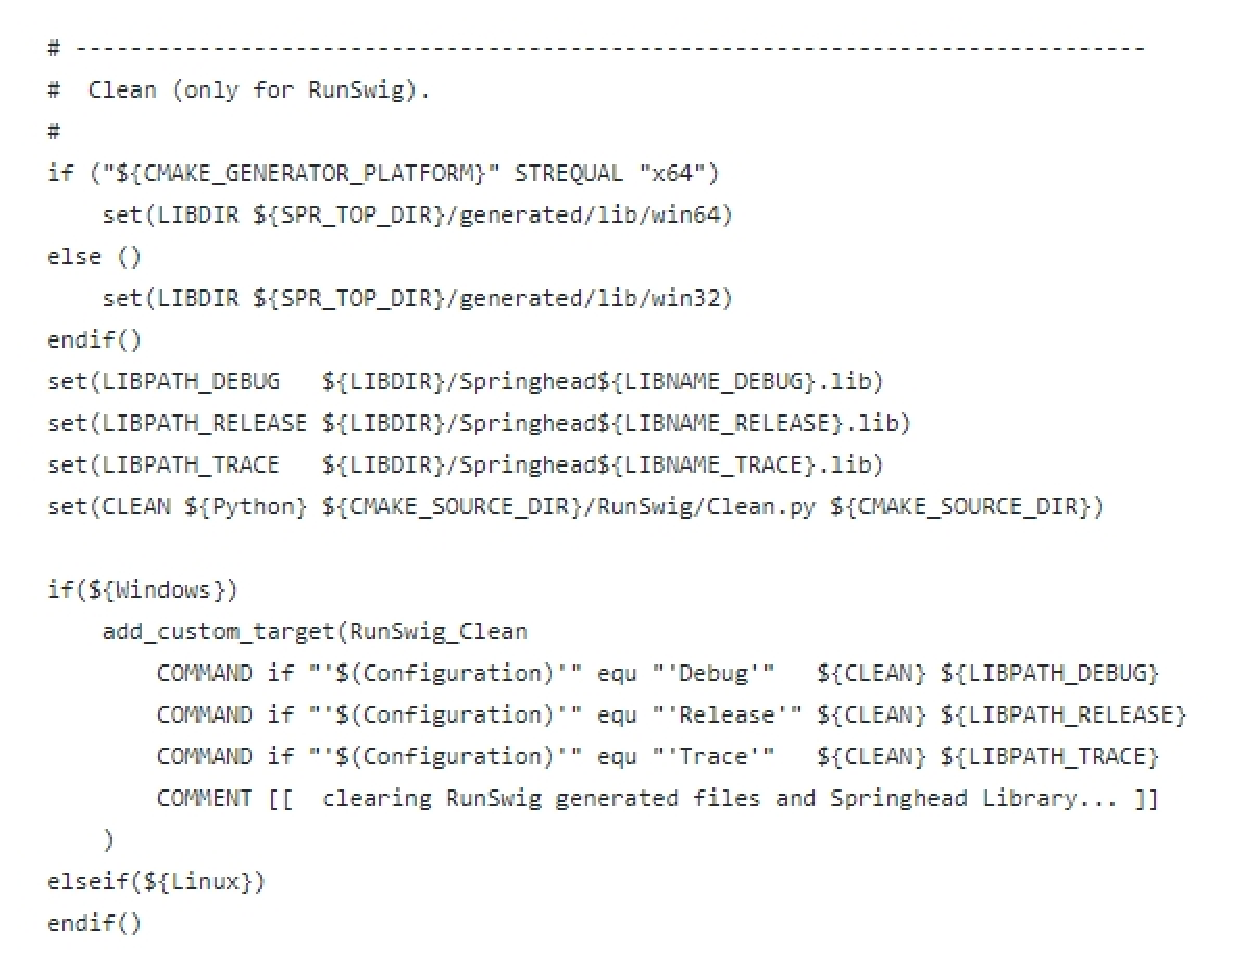
\includegraphics[width=.8\textwidth]{fig/RemoveRunSwigClean.eps}
	}\end{center}
	\label{fig:SpringheadLibraryTree}
    \end{narrow}
\end{figure}\end{narrow}
	
EmbPython\_RunSwig\_Cleanについても同様です。	

% end: 2.2.QandA.tex

% 2.3.Background.tex
%	Last update: 2020/02/13 F.Kanehori
%newpage
\subsection{補足説明}
\label{subsec:Background}
\parindent=0pt

CMakeはVisual Studio等の統合開発ツールとは異なり、
開発環境(OS)の違いおよび統合開発ツールのバージョンの違いを吸収して、
単一の制御ファイル(\QCMakeLists{})から
適切なインプットファイル(\Path{.sln}/\Path{.vcxproj},
\Path{Makefile})を自動生成するためのツールです
(unixのconfigure に近いものと考えてください)。

このため、以下に述べるような問題に対処する必要が発生します。

% end: 2.3.Background.tex

% 2.3.1.OldMethod.tex
%	Last update: 2020/02/19 F.Kanehori
%newpage
\subsubsection{従来の方法}
\label{subsubsec:OldMethod}
\parindent=0pt

Windows Visual Studioについて説明します。

\medskip
GitHubからSpringheadをダウンロードすると、
その中にライブラリをビルドするためのソリューションファイル
およびプロジェクトファイルが含まれています。

\Vskip{-.2\baselineskip}
\begin{narrow}[15pt]
	\begin{figure}[h]
	    \begin{center}
	    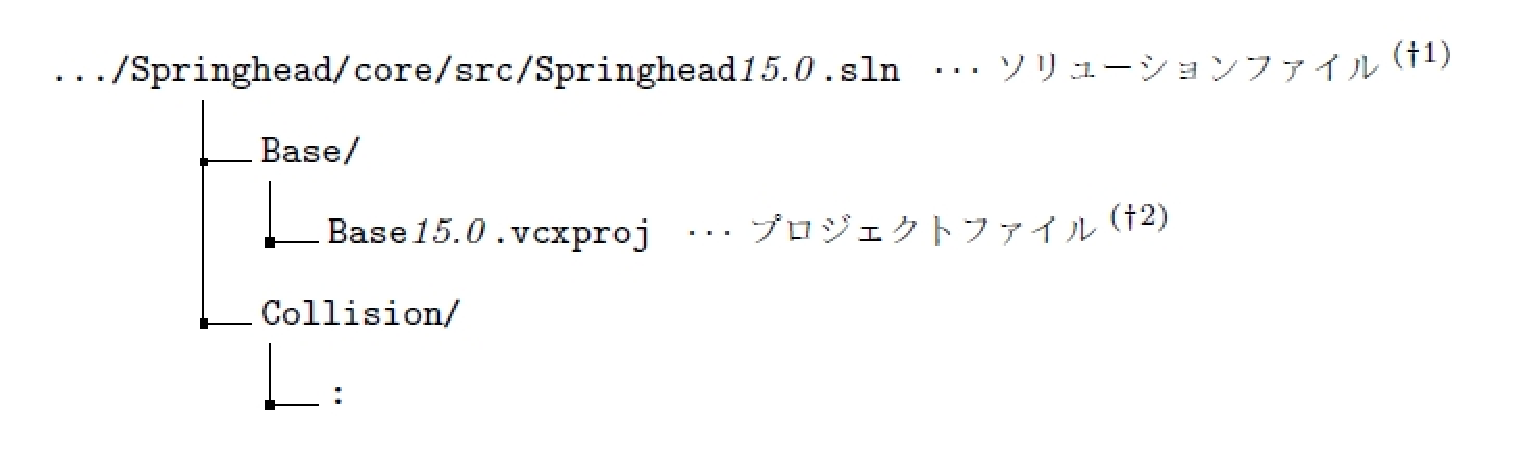
\includegraphics[width=.9\textwidth]{fig/DownloadTree.eps}
	    \end{center}
	    \label{fig:DownloadTree}
	\end{figure}
\end{narrow}
\Vskip{-.5\baselineskip}
%\begin{narrow}
%    \begin{narrow}[20pt]\begin{minipage}{\textwidth}
%	{\footnotesize{\dirtree{%
%		.1 \hspace{-10mm}C:/Springhead/core/src/Springhead\it{15.0}.sln
%			\Anno{\SolutionFile}.
%		.2 Base/.
%		.3 Base\it{15.0}.vcxproj
%			\Anno{\ProjectFile}.
%		.2 Collision/.
%		.3 :.
%	}}}
%	\medskip
%  \end{minipage}\end{narrow}
%\end{narrow}

上記の\SolutionFile を実行すればライブラリを生成することができ、
アプリケーションプログラム用のソリューションファイルに
上記の\ProjectFile を\KQuote{既存のプロジェクト}として追加すれば、
アプリケーションとライブラリの開発を同時に行なうことができました。

 後者の場合は、\ProjectFile は直接共有されることになります。このため、
\SprLib のソリューションとアプリケーション(複数でもよい)のソリューションとを
同時に開いて\ProjectFile に変更が及ぶような修正(ソースファイルの追加・削除)を
実施しても、
その変更はすべてのソリューションに直ちに反映されました。
(プロジェクトが環境外で変更された旨のダイアログが出ます)

\medskip
この方法はうまく機能していますが、次の点が難点として挙げられます。

\Vskip{-.5\baselineskip}
\begin{itemize}
  \item	Visual Studioのバージョンが変わる度に、
	ソリューションファイルとプロジェクトファイルを作り直す必要がある。
  \item	Windows以外のプラットフォームに対しては、
	Makefileなどを別途作成する必要がある。
\end{itemize}

% end: 2.3.1.OldMethod.tex

% 2.3.2.CmakeMethod.tex
%	Last update: 2020/02/32 F.Kanehori
%newpage
\subsubsection{CMakeを使用した場合}
\label{subsubsec:CmakeMethod}
\parindent=0pt

Cmakeはout of source (out of place)によるビルドに対応しています。
これはソースツリーの外側にビルドツリーを生成する機能で、次のような特徴があります。
\Vskip{-.5\baselineskip}
\begin{itemize}
  \item	互いに干渉しない複数のビルドツリーを作成することができる。
  \item	ビルドツリーが削除されてもソースツリーに影響が及ばない。
\end{itemize}
\Vskip{-.5\baselineskip}
我々はCMakeをout of sourceの方法で使用します。

\medskip
ソースツリーおよびビルドツリーは、ライブラリおよびアプリケーションのそれぞれで
次のようになるでしょう
(図\ref{fig:SpringheadLibraryTree}および図\ref{fig:ApplicationTree})。

\Vskip{-.2\baselineskip}
\begin{narrow}
    \begin{figure}[h]
	\begin{center}
	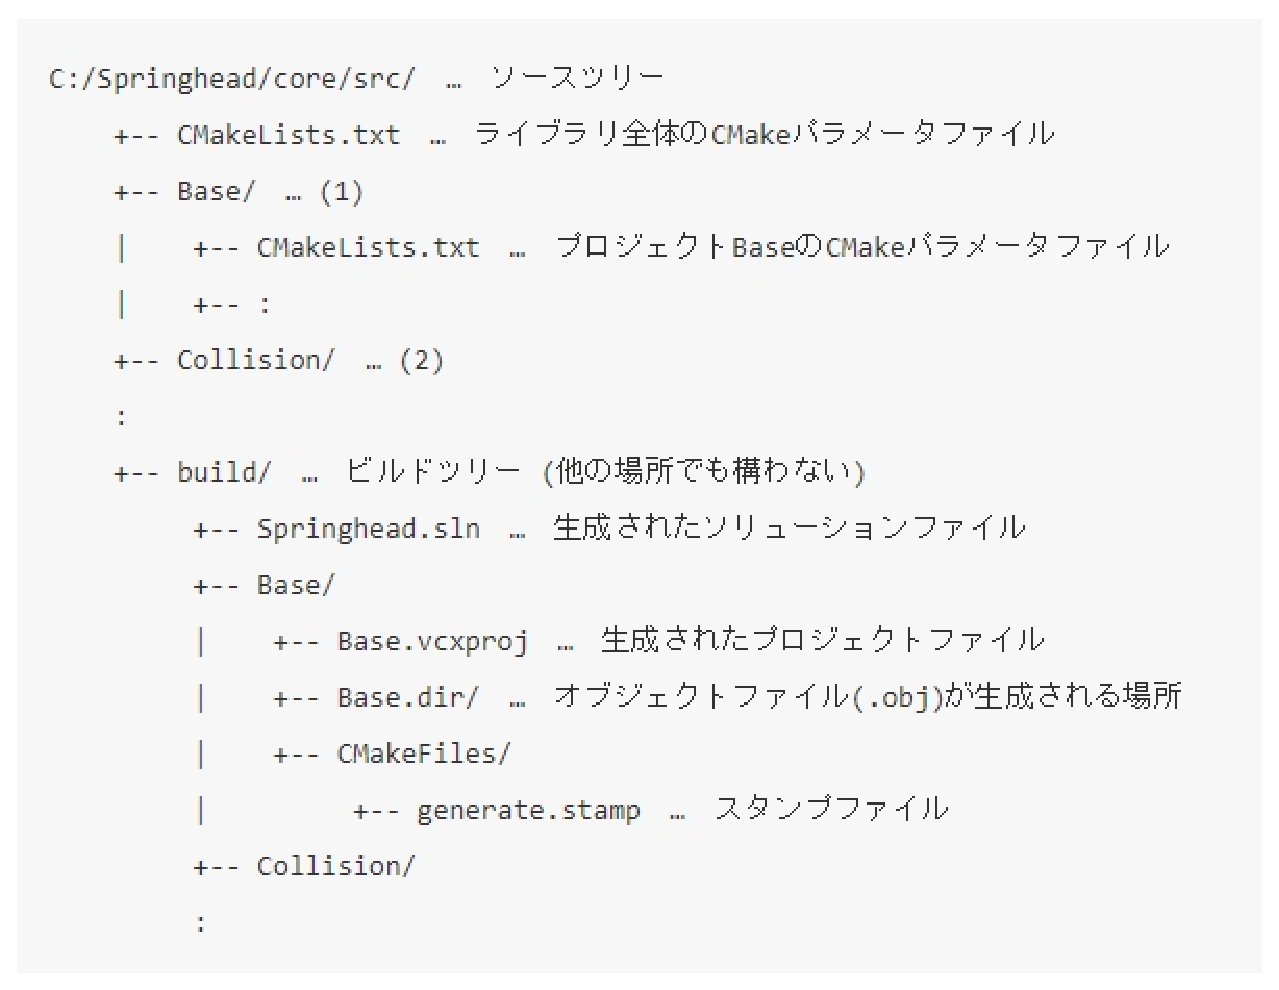
\includegraphics[width=.9\textwidth]{fig/LibraryTree.eps}
	\end{center}
	\caption{Springhead Library構成}
	\label{fig:SpringheadLibraryTree}
    \end{figure}
\end{narrow}
%\begin{narrow}\begin{figure}[h]
%    \begin{narrow}[40pt]\begin{minipage}{\textwidth}
%	{\footnotesize{\dirtree{%
%		.1 \hspace{-10mm}C:/Springhead/core/src/ \Anno{ソースツリー}.
%		.2 CMakeLists.txt \Anno{ライブラリ全体のCMakeのパラメータファイル}.
%		.2 Base/ \Anno{(1)}.
%		.3 CMakeLists.txt \Anno{プロジェクトBaseのCMakeのパラメータファイル}.
%		.3 :.
%		.2 Collision/ \Anno{(2)}.
%		.2 :.
%		.2 \BldDir \Anno{ビルドツリー (他の場所でも構わない)}.
%		.3 Springhead.sln \Anno{生成されたソリューションファイル}.
%		.3 Base/.
%		.4 Base.vcxproj \Anno{生成されたプロジェクトファイル}.
%		.4 Base.dir/ \Anno{オブジェクトファイル(\tt{.obj})が置かれる}.
%		.4 CMakeFiles/.
%		.5 generate.stamp \Anno{スタンプファイル}.
%		.3 Collision/.
%		.3 :.
%	}}}
%	\medskip
%    \end{minipage}\end{narrow}
%    \caption{Springhead Library構成}
%    \label{fig:SpringheadLibraryTree}
%\end{figure}\end{narrow}

\Vskip{-.2\baselineskip}
\begin{narrow}
    \begin{figure}[h]
	\begin{center}
	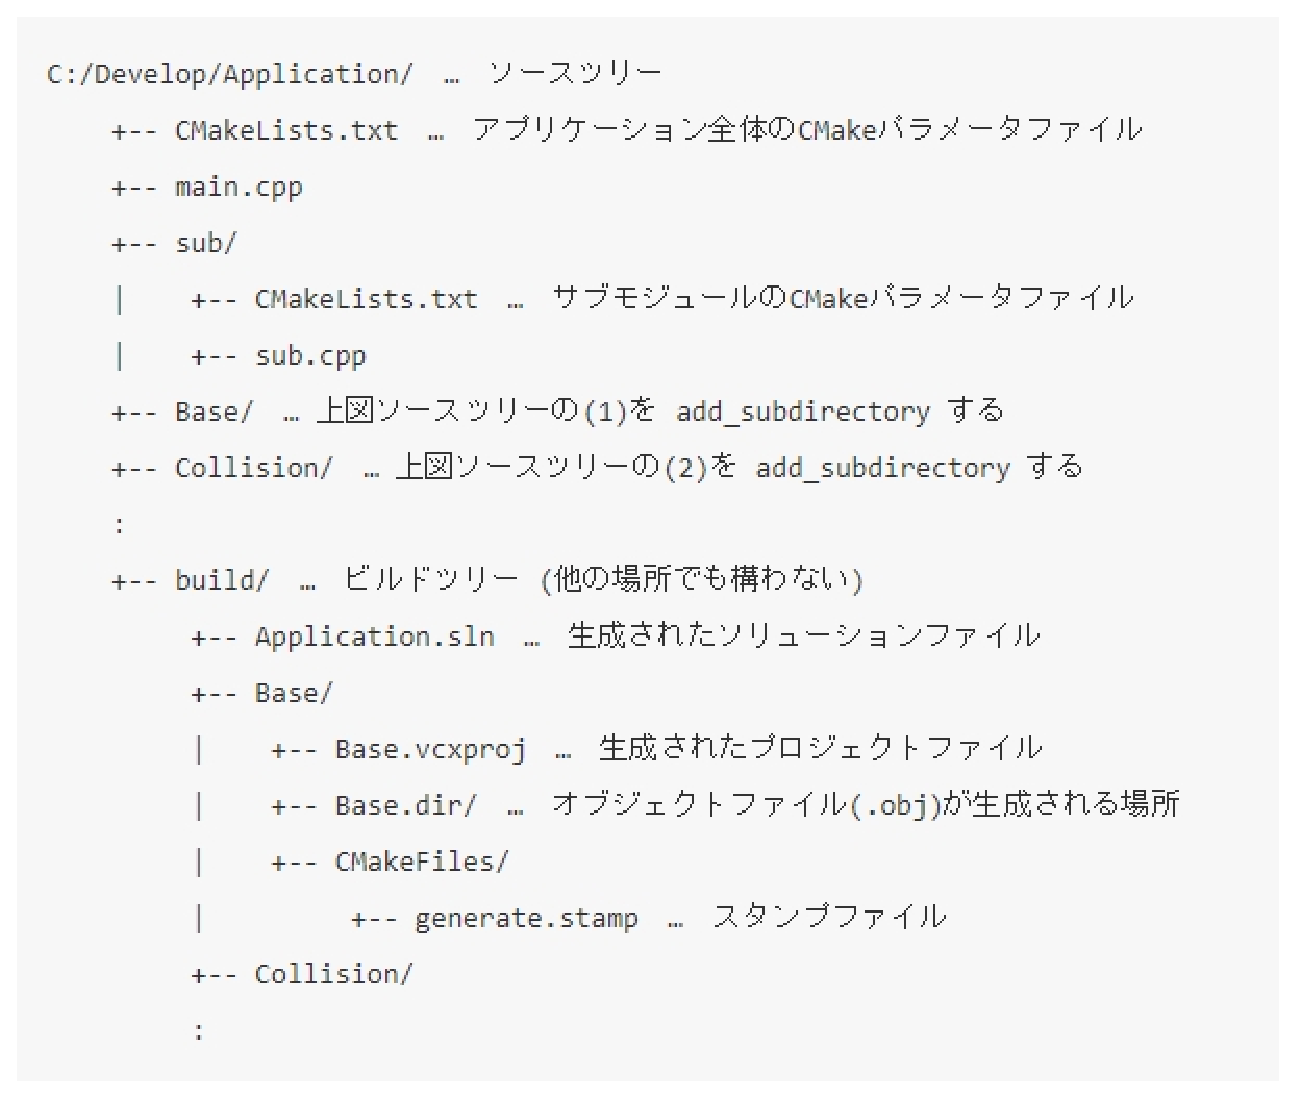
\includegraphics[width=.9\textwidth]{fig/ApplicationTree.eps}
	\end{center}
	\caption{Application構成}
	\label{fig:ApplicationTree}
    \end{figure}
\end{narrow}
%\begin{narrow}\begin{figure}[h]
%    \begin{narrow}[40pt]\begin{minipage}{\textwidth}
%	{\footnotesize{\dirtree{%
%		.1 \hspace{-10mm}C:/Develop/Application/ \Anno{ソースツリー}.
%		.2 CMakeLists.txt \Anno{アプリケーション全体のCMakeのパラメータファイル}.
%		.2 main.cpp.
%		.2 Sub/.
%		.3 CMakeLists.txt \Anno{サブモジュールのCMakeのパラメータファイル}.
%		.3 sub.cpp.
%		.2 Base/ \Anno{上図ソースツリーの(1)を\tt{add\_subdirectoryする}}.
%		.2 Collision/ \Anno{Spsringheadの(*2)を指すようにする}.
%		.2 :.
%		.2 \BldDir \Anno{ビルドツリー (他の場所でも構わない)}.
%		.3 Application.sln \Anno{生成されたソリューションファイル}.
%		.3 Base/.
%		.4 Base.vcxproj \Anno{生成されたプロジェクトファイル}.
%		.4 Base.dir/ \Anno{オブジェクトファイル(\tt{.obj})が生成される場所}.
%		.4 CMakeFiles/.
%		.5 generate.stamp \Anno{スタンプファイル}.
%		.3 Collision/.
%		.3 :.
%	}}}
%	\medskip
%    \end{minipage}\end{narrow}
%    \caption{Application構成}
%    \label{fig:ApplicationTree}
%\end{figure}\end{narrow}

\medskip
ライブラリをビルドしたときもアプリケーションをビルドしたときも、
それぞれのビルドにおける生成物は、
すべてそれぞれのビルドツリー内におかれることに注意してください。
言い換えると、 ライブラリのオブジェクトファイルが、
複数のビルドツリーに独立して配置されるということです。

% end: 2.3.2.CmakeMethod.tex

% 2.3.3.Problems.tex
%	Last update: 2020/02/13 F.Kanehori
%newpage
\subsubsection{問題点}
\label{subsubsec:Problems}
\parindent=0pt

\def\App#1{\it{App#1\,}}
\def\App#1{\it{App#1\,}}

前節\KQuote{\ref{subsubsec:CmakeMethod}CMakeを使用した場合} に示したような
アプリケーション\App{1}の他にアプリケーション\App{2}があったとして、
その両方を同時に開いて作業を行なう場合を考えます。
ここでは\App{1}と\App{2}が共通して参照する\SprLib のプロジェクトについてのみ考えます。

\bigskip
\bf{ソースファイルの整合性}
\begin{narrow}[20pt]
	ソースファイルの整合性には問題がありません。
	\App{1}と\App{2}のどちらも\SprLib のソースツリーを指すようにしてありますから、
	どちらで実施したソースファイルの変更も直ちに他方に反映されることになります。
	(同じファイルを参照しているのですから当然です)

	\medskip
	ソースファイルの追加や削除を実施したとしても
	ソースファイルの整合性自体が崩れるわけではありません。
	ただし、この場合には\KQuote{\bf{プロジェクトファイルの整合性}}(後述)
	の問題が発生します。
\end{narrow}

\medskip
\bf{ビルドの最適性(無駄なコンパイル)}
\begin{narrow}[20pt]
	\App{1}と\App{2}のビルドツリーは異なるものですから、
	\App{1}でソースを変更してビルドしたとしても
	そのビルド結果(オブジェクトファイル)がそのまま\App{2}から見える訳ではありません。

	\medskip
	\App{2}でこの変更を反映させようとすれば\App{2}での再ビルドが必要ですが、
	再ビルドを行なった時点で初めて変更されたソースファイルが再コンパイルされ、
	オブジェクトファイルの整合性がとれることになります。
	従来はオブジェクトファイルも共有されていましたから、
	このような無駄なコンパイルは発生しませんでした。
\end{narrow}

\medskip
\bf{プロジェクトファイルの整合性 --- Windows (Visual Studio)の場合}
\label{subsec:Problems:ProjectFileIntegration}
\begin{narrow}[20pt]
	ソースファイルの内容を修正しただけならば
	プロジェクトファイルが変更されることはありません。
	しかし、ソースファイルの追加や削除を行なったならば
	プロジェクトファイルにも変更が及びます
	(Visual Studio上でソースの追加・削除を行なってセーブを行なった場合、
	もしくは\App{1}での変更後に再\cmake を行なった場合)。

	\medskip
	プロジェクトファイルもオブジェクトファイルと同様に
	ビルドツリー内に生成されますから、
	\App{1}で実施した変更が
	異なるビルドツリーをもつ\App{2}に反映されることはありません。
	しかも\App{2}で再ビルドしたとしても\App{1}での変更が反映されることはありません。
	\App{2}のプロジェクトファイルは\App{1}のものとは異なるファイルですから
	\App{2}は依然として古い状態を残したままなのです。

	\medskip
	これを解消するには\App{2}で再度\cmake を実行する必要がありますが、
	問題は\KQuote{\bf{いつ再\cmake が必要なのかが分からない}}ということです。
\end{narrow}

% end: 2.3.3.Problems.tex

% 2.3.4.Solutions.tex
%	Last update: 2020/03/30 F.Kanehori
%newpage
\subsubsection{対処法}
\label{subsubsec:Solutions}
\parindent=0pt

前節で示した問題点への対処法について述べます。

\bigskip
\bf{ソースファイルの整合性}
\begin{narrow}[20pt]
	\SprLib のソースツリーにあるプロジェクトディレクトリ
	(Base, Collision, ...)を直接`\tt{add\_subdirectory}'すれば十分です。
\end{narrow}

\medskip
\bf{ビルドの最適性(無駄なコンパイル)}
\begin{narrow}[20pt]
	\SprLib, \it{App1, App2\,}などのすべてにおいて、
	ライブラリのオブジェクトが生成される場所を共通化してしまうことで
	この問題を回避することとします。
	具体的には、\SprLib ソースツリーの中(ビルドツリーの外)に
	オブジェクトの共通格納場所を作り、
	\SprLib およびすべてのアプリケーションで、
	ライブラリのオブジェクト格納ディレクトリをそこへのlinkとします。

	\begin{figure}[h]
	    \begin{center}
	    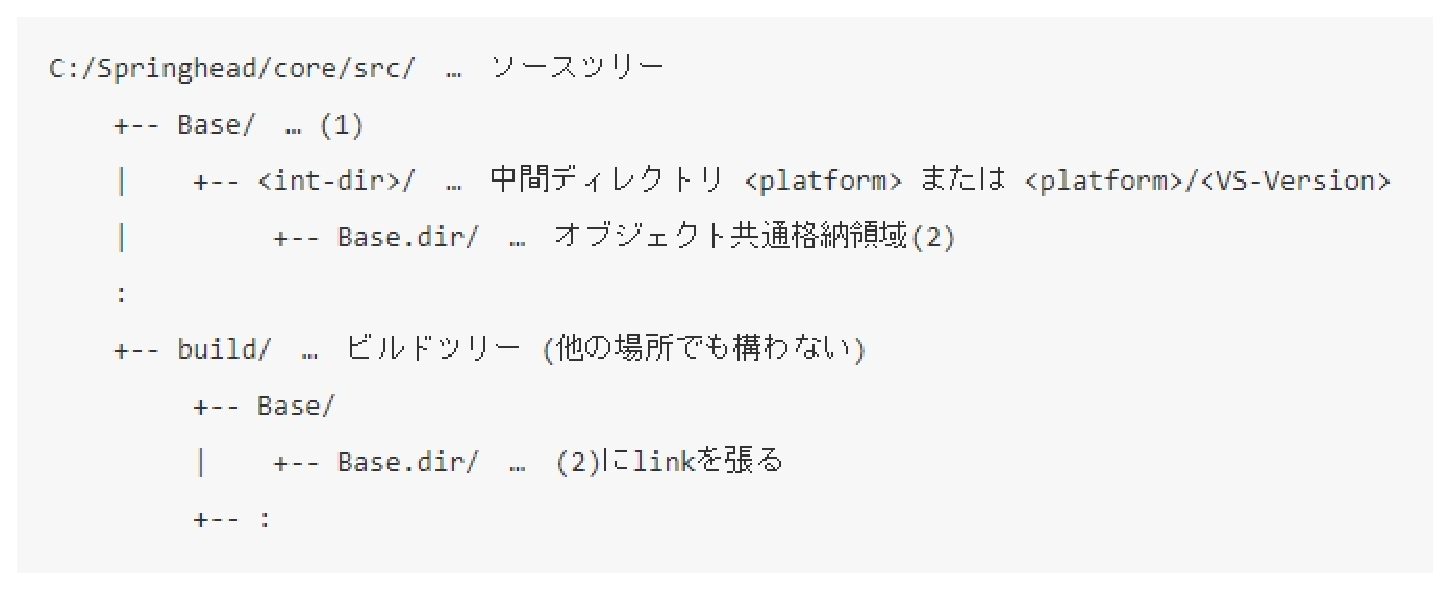
\includegraphics[width=1\textwidth]{fig/ApproachToBuildOptimization-1.eps}
	    \end{center}
	\end{figure}
	\Vskip{-.5\baselineskip}
	\begin{figure}[h]
	    \begin{center}
	    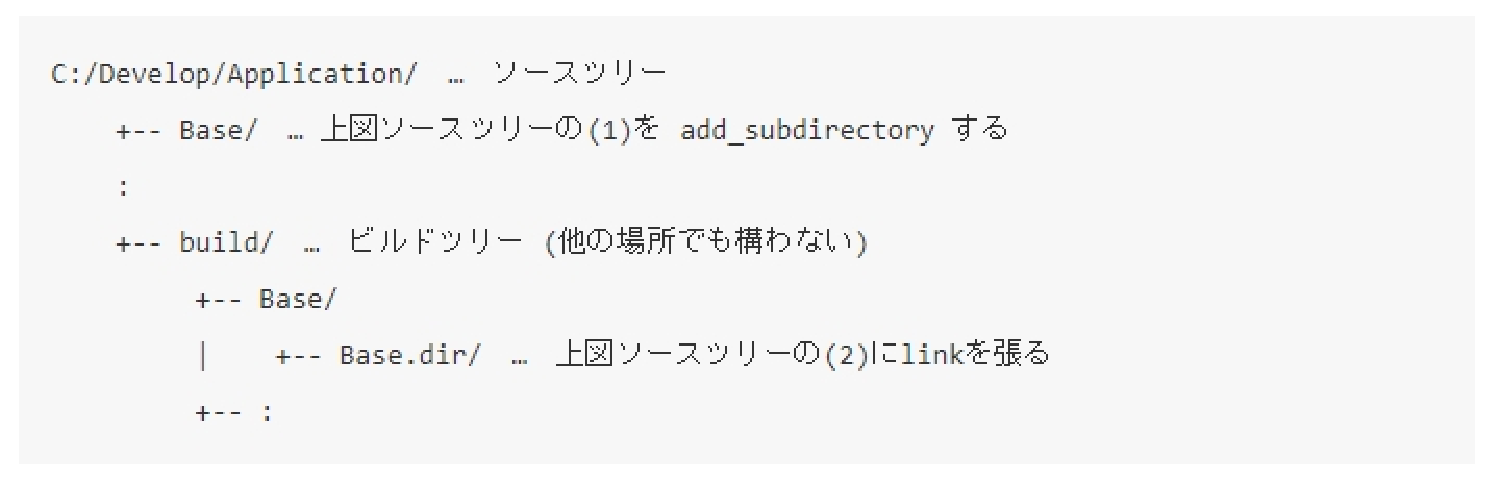
\includegraphics[width=1\textwidth]{fig/ApproachToBuildOptimization-2.eps}
	    \end{center}
	    \caption{ビルドの最適性への対処法}
	    \label{fig:ApproachToBuildOptimization}
	\end{figure}
%	\begin{figure}[h]
%    	\begin{narrow}[40pt]\begin{minipage}{\textwidth}
%		{\footnotesize{\dirtree{%
%			.1 \hspace{-10mm}C:/Springhead/core/src/ \Anno{ソースツリー}.
%			.2 Base/ \Anno{(1)}.
%			.3 <\it{int-dir\,}>/
%				\Anno{中間ディレクトリ <platform>
%					または<platform>/<VS-Version>}.
%			.4 Base.dir/ \Anno{オブジェクト共通格納領域(2)}.
%			.3 :.
%			.2 :.
%			.2 \BldDir \Anno{ビルドツリー (他の場所でも構わない)}.
%			.3 Base/.
%			.4 Base.dir/ \Anno{(2)にlinkを張る}.
%			.2 :.
%		}}}
%		\medskip
%    	\end{minipage}\end{narrow}
%    	\begin{narrow}[40pt]\begin{minipage}{\textwidth}
%		{\footnotesize{\dirtree{%
%			.1 \hspace{-10mm}C:/Develop/Application/ \Anno{ソースツリー}.
%			.2 Base/
%				\Anno{上図ソースツリーの(1)を\tt{add\_subdirectory}する}.
%			.2 :.
%			.2 \BldDir \Anno{ビルドツリー (他の場所でも構わない)}.
%			.3 Base/.
%			.4 Base.dir/ \Anno{上図ソースツリーの(2)にlinkを張る}.
%			.3 :.
%		}}}
%		\medskip
%  	\end{minipage}\end{narrow}
%	\caption{ビルドの最適性への対処法}
%	\label{fig:ApproachToBuildOptimization}
%	\end{figure}

	\medskip
	オブジェクトの共通格納領域を設定する作業は\SprLib の\cmake\ (configure)時に、
	linkを張る作業はアプリケーションの\cmake\ (configure)時に行なうものとします。
\end{narrow}

\medskip
\bf{プロジェクトファイルの整合性 (Visual Studioの場合)}
\begin{narrow}[20pt]
	ビルドの最適性の場合と同様、
	ソリューションファイルおよびプロジェクトファイルを共通化することで
	この問題に対処します。
	具体的には、\SprLib ビルドツリー上にあるものを最新の状態に保つことを前提として、
	すべてのアプリケーションについて、
	\SprLib のプロジェクトに関わるソリューションファイル
	およびプロジェクトファイルはすべて
	\SprLib ビルドツリーにあるものの複製をもつようにします。

	\medskip
	ただしこれでは不完全で、\App{1}で実施したプロジェクトファイルへの変更が
	\App{2}に伝わりません。
	このため\App{1}でプロジェクトファイルを変更した場合には、
	その変更内容を\SprLib ビルドツリーにあるプロジェクトファイルにコピーすることで、
	\SprLib のビルドツリーにあるプロジェクトファイルが
	常に最新のものであることを保証します。

	\medskip
	この作業はアプリケーションのビルド時に行なうものとします。
	そのために、各アプリケーションのソリューションファイルに
	特別なターゲット`\tt{sync}'を作成し、
	このターゲットが毎回のビルドに先立って実行されるようにします。

	\begin{figure}[h]
	    \begin{center}
	    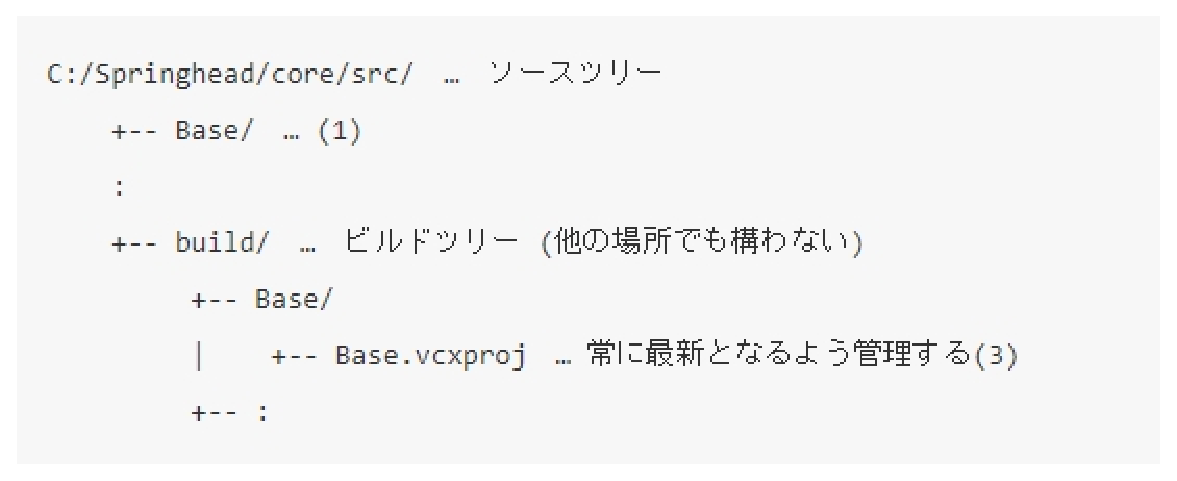
\includegraphics[width=.85\textwidth]{fig/ApproachToProjfileOptimization-1.eps}
	    \end{center}
	\end{figure}
	\Vskip{-.5\baselineskip}
	\begin{figure}[h]
	    \begin{center}
	    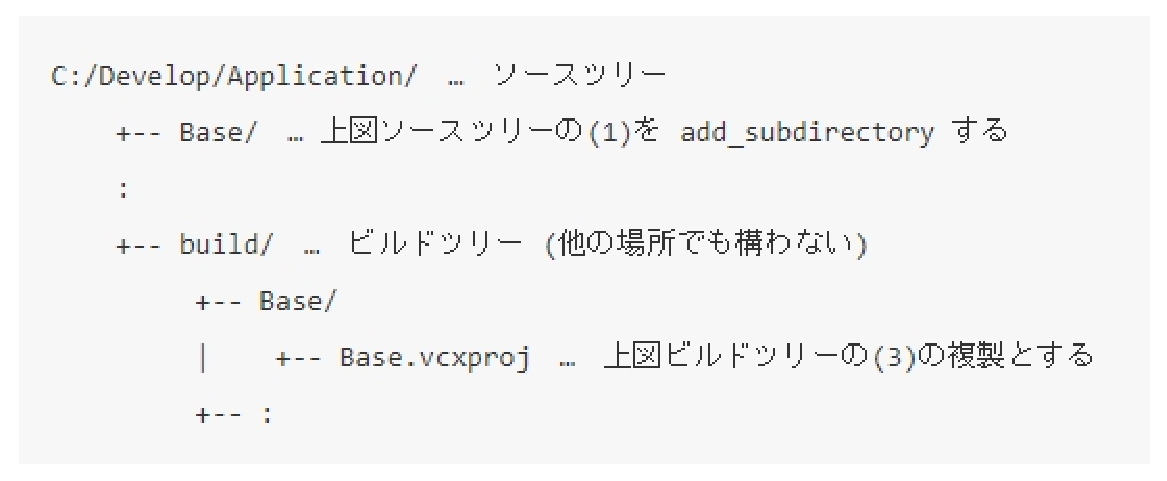
\includegraphics[width=.85\textwidth]{fig/ApproachToProjfileOptimization-2.eps}
	    \end{center}
	    \caption{プロジェクトファイルの最適性への対処法}
	    \label{fig:ApproachToProjfileOptimization}
	\end{figure}
%	\begin{figure}[h]
%    	\begin{narrow}[40pt]\begin{minipage}{\textwidth}
%		{\footnotesize{\dirtree{%
%			.1 \hspace{-10mm}C:/Springhead/core/src/ \Anno{ソースツリー}.
%			.2 Base/ \Anno{(1)}.
%			.2 :.
%			.2 \BldDir \Anno{ビルドツリー (他の場所でも構わない)}.
%			.3 Base/.
%			.4 Base.vcxproj \Anno{常に最新となるように管理する(3)}.
%			.2 :.
%		}}}
%		\medskip
%    	\end{minipage}\end{narrow}
%    	\begin{narrow}[40pt]\begin{minipage}{\textwidth}
%		{\footnotesize{\dirtree{%
%			.1 \hspace{-10mm}C:/Develop/Application/ \Anno{ソースツリー}.
%			.2 Base/ \Anno{上図ソースツリーの(1)を\tt{add\_subdirectory}する}.
%			.2 :.
%			.2 \BldDir \Anno{ビルドツリー (他の場所でも構わない)}.
%			.3 Base/.
%			.4 Base.vcxprj/ \Anno{上図ビルドツリーの(3)の複製とする}.
%			.3 :.
%		}}}
%		\medskip
%  	\end{minipage}\end{narrow}
%	\caption{プロジェクトファイルの最適性への対処法}
%	\label{fig:ApproachToProjfileOptimization}
%	\end{figure}
\end{narrow}

% end: 2.3.4.Solutions.tex

% 2.3.5.Implementation.tex
%	Last update: 2020/02/13 F.Kanehori
%newpage
\subsubsection{実装}
\label{subsubsec:Implementation}
\parindent=0pt

この節では、\KQuote{\ref{subsubsec:Solutions} 対処法}の実装に関する補足説明をします。

\medskip
\bf{ソースファイルの整合性}
\begin{narrow}
	\QCMakeLists{}に組み込みます
	(\QCMakeSettings{}の\tt{SPR\_PROJS}で定義したプロジェクトのすべてを
	\tt{add\_subdirectory}します)。\\
	\QCMakeLists{.Dev.dist}を参照のこと。
\end{narrow}

\medskip
\bf{ビルドの最適性(無駄なコンパイル)}
\begin{narrow}
	組み込まれる\SprLib の各プロジェクトに対して、
	次のことを実施します (ここではBaseを例に説明します)。

	\medskip
	\cmake (configure)実行時に作成されるオブジェクト格納ディレクトリ\\
	\hspace{10pt}\Path{C:/Develop/Application/build/Base/Base.dir}\\
	を、オブジェクト共通格納場所\\
	\hspace{10pt}\Path{C/Springhead/core/src/Base/<\it{platform}>/<\it{VS-Version}>/Base.dir}\\
	へのlink(*)にすげ替えます。

	\medskip
	オブジェクト共通格納場所は、\SprLib の\cmake (configure) 時に作成します。
	各プロジェクトの\QCMakeLists{}から
	\tt{execute\_process}で呼び出される\Path{make\_prconfig.py}を参照のこと。

	\medskip
	\Important{%
		ここで作成するlinkは、unixではsymbolic link、Windowsではjunctionです。
		これは、
		Windowsでは通常の実行権限ではsymblic linkが作成できないためです。\\
		Windowsでは、\Path{Base.dir}がjunctionなのか通常のディレクトリなのかが、
		explorerでもcommand promptでも区別がつきません。
		このことが、Q\&Aの\KQuote{\ref{subsec:QandA:CrumbleBuildOptimizeation}
		ビルドの最適性が崩れる}の原因究明を困難にする可能性を孕んでいます。
		ここでは、
		オブジェクト共通格納場所には`\tt{\_target\_body\_}'という名前の
		空ファイルを 置くことで判定の補助としています。}
\end{narrow}

\medskip
\bf{プロジェクトファイルの整合性(Visual Studio の場合)}
\begin{narrow}
	アプリケーションのソリューションファイルに新たなターゲットsyncを追加して、
	次の処理を順に実行させます。
	これにより、\SprLib 側または他のアプリケーションが実施した変更は、
	アプリケーションをビルドするだけで自動的に反映されます。

	\begin{enumerate}
	  \item	もしもアプリケーション側のプロジェクトファイルの内容と\SprLib 側の
		プロジェクトファイルの内容とが異なっていたならば、
		アプリケーション側のプロジェクトファイルを\SprLib 側にコピーする。
		これは、アプリケーション側でソースファイル構成を変更(追加・削除)を行ない、
		Visual Studio上でプロジェクトファイルを保存したとき、
		またはアプリケーション側で再度\cmake を実行した場合に相当します。

	  \item	\SprLib 側のプロジェクトファイルをアプリケーション側にコピーする。
	\end{enumerate}

	ターゲットsyncは、アプリケーションの\QCMakeLists{}で
	\tt{add\_custom\_target}として作成されます。
	また、このターゲットはアプリケーションのビルドにおいて
	必ず最初に実行されるように依存関係が設定されます。
	\QCMakeLists{.Dev.dist}および\tt{"make\_sync.py"}を参照のこと。

	\medskip
	\Important{%
		自アプリケーションで実施したソース構成の変更は、
		ビルドを実施した時点で\SprLib 側に反映されます。
		つまり、プロジェクトファイルの整合性を保つためには、
		ソース構成の変更後に少なくとも1回はビルドを実行する必要があるということです
		(syncの実行だけでもよい)。
		しかしソースを変更したならばビルドするでしょうから、
		このことが問題になることはないでしょう。}
\end{narrow}

% end: 2.3.5.Implementation.tex




\ifLwarp
  %\begin{warpprint}   % For print output ...
  %  \cleardoublepage    % ... a common method to place index entry into TOC.
  %  \phantomsection
  %  \addcontentsline{toc}{chapter}{\indexname}
  %\end{warpprint}
  \ForceHTMLPage      % HTML index will be on its own page.
  \ForceHTMLTOC       % HTML index will have its own toc entry.
  \printindex
\fi


\end{document}
